\flushbottom











%%============================================================================
%%============================================================================
\chapter{Bessel Functions}
\index{Bessel functions}
\index{Bessel's equation}



Ideas are angels.  Implementations are a bitch.








%%===========================================================================
\section{Bessel's Equation}



A commonly encountered differential equation in applied mathematics is 
\textit{Bessel's equation}
\[ 
y'' + \frac{1}{z} y' + \left( 1 - \frac{\nu^2}{z^2} \right)y = 0.
\]
For our purposes, we will consider $\nu \in \mathbb{R}^{0+}$.
This equation arises when solving certain partial differential equations
with the method of separation of variables
in cylindrical coordinates.  For this reason, the solutions of this
equation are sometimes called \textit{cylindrical functions}.

This equation cannot be solved directly.  However, we can
find series representations of the solutions.  There is a regular singular
point at $z = 0$, so the Frobenius method is applicable there.
The point at infinity is an irregular singularity, so we will look
for asymptotic series about that point.  
Additionally, we will use Laplace's method to find definite integral
representations of the solutions.

Note that Bessel's equation depends only on $\nu^2$ and not $\nu$ alone.
Thus if we find a solution, (which of course depends on this parameter),
$y_\nu(z)$ we know that $y_{-\nu}(z)$ is also a solution.  For this 
reason, we will consider $\nu \in \mathbb{R}^{0+}$.
Whether or not $y_\nu(z)$ and $y_{-\nu}(z)$ are linearly independent,
(distinct solutions), remains to be seen.


\begin{Example}
  Consider the differential equation
  \[
  y'' + \frac{1}{z} y' + \frac{\nu^2}{z^2} y = 0
  \]
  One solution is $y_\nu(z) = z^\nu$.  Since the equation depends only 
  on $\nu^2$, another solution is $y_{-\nu}(z) = z^{-\nu}$.  For 
  $\nu \neq 0$, these two solutions are linearly independent.

  Now consider the differential equation
  \[
  y'' + \nu^2 y = 0
  \]
  One solution is $y_\nu(z) = \cos(\nu z)$.  Therefore,
  another solution is $y_{-\nu}(z) = \cos(-\nu z) = \cos(\nu z)$.
  However, these two solutions are not linearly independent.
\end{Example}





%%===========================================================================
\section{Frobeneius Series Solution about z = 0}

We note that $z=0$ is a regular singular point, (the only
singular point of Bessel's equation in the finite complex plane.)  
We will use the Frobenius method at that point to analyze the solutions.
We assume that $\nu \geq 0$.

The indicial equation is 
\begin{gather*}
  \alpha(\alpha-1) + \alpha - \nu^2 = 0 \\
  \alpha = \pm \nu.
\end{gather*}
If $\pm \nu$ do not differ by an integer, (that is if $\nu$ is not a 
half-integer), then there will be two series solutions of the Frobenius 
form.
\[
y_1(z) = z^\nu \sum_{k = 0}^\infty a_k z^k, 
\quad
y_2(z) = z^{-\nu} \sum_{k = 0}^\infty b_k z^k 
\]
If $\nu$ is a half-integer, the second solution may or may not be in the
Frobenius form.  In any case, then will always be at least one solution 
in the Frobenius form.  We will determine that series solution.
$y(z)$ and it derivatives are
\[
y = \sum_{k = 0}^\infty a_k z^{k+\nu}, \quad
y' = \sum_{k = 0}^\infty (k + \nu) a_k z^{k+\nu-1}, \quad
y'' = \sum_{k = 0}^\infty (k + \nu)(k + \nu - 1) a_k z^{k+\nu-2}.
\]

We substitute the Frobenius series into the differential equation.
\begin{gather*}
  z^2 y'' + z y' + \left( z^2 - \nu^2 \right) y = 0 \\
  \sum_{k = 0}^\infty (k + \nu)(k + \nu - 1) a_k z^{k+\nu}
  + \sum_{k = 0}^\infty (k + \nu) a_k z^{k+\nu} + \sum_{k = 0}^\infty a_k z^{k+\nu+2}
  - \sum_{k = 0}^\infty \nu^2 a_k z^{k+\nu} = 0 \\
  \sum_{k = 0}^\infty \left( k^2 + 2 k \nu \right) a_k z^{k}
  + \sum_{k=2}^\infty a_{k-2} z^k = 0
\end{gather*}
We equate powers of $z$ to obtain equations that determine the coefficients.
The coefficient of $z^0$ is the equation $0 \cdot a_0 = 0$.
This corroborates that $a_0$ is arbitrary, (but non-zero).
The coefficient of $z^1$ is the equation
\begin{gather*}
  (1 + 2 \nu) a_1 = 0 \\
  a_1 = 0
\end{gather*}
The coefficient of $z^k$ for $k \geq 2$ gives us
\begin{gather*}
  \left( k^2 + 2 k \nu \right) a_k + a_{k-2} = 0. \\
  a_k = - \frac{a_{k-2}}{ k^2 + 2 k \nu } = - \frac{a_{k-2}}{ k (k + 2 \nu) }
\end{gather*}
From the recurrence relation we see that all the odd coefficients are zero,
$a_{2k+1} = 0$.  The even coefficients are
\[
a_{2 k} = - \frac{ a_{2k-2} }{ 4 k (k + \nu) }
= \frac{ (-1)^k a_0 }{ 2^{2k} k! \Gamma(k + \nu + 1) }
\]
Thus we have the series solution
\[
y(z) = a_0 \sum_{k = 0}^\infty \frac{ (-1)^k }{ 2^{2k} k! \Gamma(k + \nu + 1) }
z^{2k}.
\]
$a_0$ is arbitrary.  We choose $a_0 = 2^{-\nu}$.
We call this solution the \textit{Bessel function of the first kind
  and order $\nu$} and denote it with $J_\nu(z)$.
\[
J_\nu(z) = \sum_{k = 0}^\infty \frac{ (-1)^k }{ k! \Gamma(k + \nu + 1) }
\left( \frac{z}{2} \right)^{2 k + \nu}
\]

%% CONTINUE HERE

Recall that the Gamma function is non-zero and finite for all real arguments
except non-positive integers.  $\Gamma(x)$ has singularities at 
$x = 0, -1, -2, \ldots$.  Therefore, $J_{-\nu}(z)$ is well-defined
when $\nu$ is not a positive integer.  Since $J_{-\nu}(z) \sim z^{-\nu}$
at $z = 0$, $J_{-\nu}(z)$ is clear linearly independent to $J_\nu(z)$
for non-integer $\nu$.  In particular we note that there are two solutions
of the Frobenius form when $\nu$ is a half odd integer.
\[
J_{-\nu}(z) = \sum_{k = 0}^\infty \frac{ (-1)^k }{ k! \Gamma(k - \nu + 1) }
\left( \frac{z}{2} \right)^{2 k - \nu}, 
\quad \mathrm{for}\ \nu \not \in \mathbb{Z}^+
\]

Of course for $\nu = 0$, $J_\nu(z)$ and $J_{-\nu}(z)$ are identical.
Consider the case that $\nu = n$ is a positive integer.  Since 
$\Gamma(x) \to +\infty$ as $x \to 0, -1, -2, \ldots$ we see the the 
coefficients in the series for $J_{-nu}(z)$ vanish for 
$k = 0, \ldots, n-1$.
\begin{gather*}
  J_{-n}(z) = \sum_{k = n}^\infty \frac{ (-1)^k }{ k! \Gamma(k - n + 1) }
  \left( \frac{z}{2} \right)^{2 k - n} \\
  J_{-n}(z) = \sum_{k = 0}^\infty \frac{ (-1)^{k+n} }{ (k+n)! \Gamma(k + 1) }
  \left( \frac{z}{2} \right)^{2 k + n} \\
  J_{-n}(z) = (-1)^n \sum_{k = 0}^\infty \frac{ (-1)^k }{ k! (k+n)! }
  \left( \frac{z}{2} \right)^{2 k + n} \\
  J_{-n}(z) = (-1)^n J_n(z)
\end{gather*}
Thus we see that $J_{-n}(z)$ and $J_n(z)$ are not linearly independent 
for integer $n$.






%%===========================================================================
\subsection{Behavior at Infinity}



With the change of variables $z = 1/\zeta$, $w(z) = u(\zeta)$ Bessel's equation
becomes
\begin{gather*}
  \zeta^4 u'' + 2 \zeta^3 u' + \zeta \left( - \zeta^2 \right) u'+ \left( 1 - \nu^2 \zeta^2 \right) u = 0 
  \\
  u'' + \frac{1}{\zeta} u' + \left(\frac{1}{\zeta^4} - \frac{\nu^2}{\zeta^2}\right)u = 0.
\end{gather*}
The point $\zeta = 0$ and hence the point $z = \infty$ is an irregular singular
point.  We will find the leading order asymptotic behavior of the solutions
as $z \to +\infty$.


\paragraph{Controlling Factor.}
We starti with Bessel's equation for real argument.
\[ 
y'' + \frac{1}{x} y' + \left(1 - \frac{\nu^2}{x^2} \right) y = 0
\]
We make the substitution $y = \e^{s(x)}$.
\[
s'' + (s')^2 + \frac{1}{x} s' + 1 - \frac{\nu^2}{x^2} = 0
\] 
We know that $\frac{\nu^2}{x^2} \ll 1$ as $x \to \infty$;  we will assume
that $s'' \ll (s')^2$ as $x \to \infty$.
\[ 
(s')^2 + \frac{1}{x} s' + 1 \sim 0 \quad \mathrm{as}\ x \to \infty
\]
To simplify the equation further, we will try the possible two-term balances.
\begin{enumerate}
\item
  $(s')^2 + \frac{1}{x} s' \sim 0 \quad \to \quad s' \sim -\frac{1}{x} \qquad$
  This balance is not consistent as it violates the assumption that
  $1$ is smaller than the other terms.
\item
  $(s')^2 + 1 \sim 0 \quad        \to \quad      s' \sim \pm \imath \qquad$
  This balance is consistent.
\item
  $\frac{1}{x} s' + 1 \sim 0 \quad \to \quad s' \sim -x \qquad$
  This balance is inconsistent as $(s')^2$ isn't smaller than the other terms.
\end{enumerate}

Thus the only dominant balance is $s' \sim \pm \imath$.  
This balance is consistent with our initial assumption that $s'' \ll (s')^2$.
Thus $s \sim \pm \imath x$ and the controlling factor is $\e^{\pm \imath x}$.




\paragraph{Leading Order Behavior.}
In order to find the leading order behavior, we substitute $s = \pm \imath x 
+ t(x)$ where $t(x) \ll x$ as $x \to \infty$ into the differential equation
for $s$.  We first consider the case $s = \imath x + t(x)$.
We assume that $t' \ll 1$ and $t'' \ll 1/x$.
\begin{gather*}
  t'' + (\imath + t')^2 + \frac{1}{x}(\imath + t') + 1 - \frac{\nu^2}{x^2} = 0 
  \\
  t'' + \imath 2 t' + (t')^2 + \frac{\imath}{x} + \frac{1}{x} t' - \frac{\nu^2}{x^2} = 0
  \\
  \intertext{We use our assumptions about the behavior of $t'$ and $t''$.}
  \imath 2 t' + \frac{\imath}{x} \sim 0 
  \\
  t' \sim -\frac{1}{2 x} \\
  t \sim - \frac{1}{2} \ln x \quad \mathrm{as}\ x \to \infty.
\end{gather*}
This asymptotic behavior is consistent with our assumptions.

Substituting $s = - \imath x + t(x)$ will also yield $t \sim -\frac{1}{2} \ln x$.
Thus the leading order behavior of the solutions is
\[ 
y \sim c \e^{\pm \imath x - \frac{1}{2} \ln x + u(x)} 
= c x^{-1/2} \e^{\pm \imath x + u(x)} \quad \mathrm{as}\ x \to \infty,
\]
where $u(x) \ll \ln x$ as $x \to \infty$.

By substituting $t = -\frac{1}{2} \ln x + u(x)$ into the differential equation
for $t$, you could show that $u(x) \to $ const as $x \to \infty$.  Thus the
full leading order behavior of the solutions is
\[ 
y \sim c x^{-1/2} \e^{\pm \imath x + u(x)} \quad \mathrm{as}\ x \to \infty
\]
where $u(x) \to 0$ as $x \to \infty$.
Writing this in terms of sines and cosines yields
\[ 
y_1 \sim x^{-1/2} \cos(x + u_1(x)), \qquad
y_2 \sim x^{-1/2} \sin(x + u_2(x)), \quad \mathrm{as}\ x \to \infty,
\]
where $u_1,u_2 \to 0$ as $x \to \infty$.




\begin{Result}
  Bessel's equation for real argument is
  \[ 
  y'' + \frac{1}{x} y' + \left( 1 - \frac{\nu^2}{x^2} \right) y = 0.
  \]
  If $\nu$ is not an integer then the solutions behave as linear combinations
  of
  \[ 
  y_1 = x^\nu, \quad \mathrm{and} \quad y_2 = x^{-\nu}
  \]
  at $x = 0$.
  If $\nu$ is an integer, then the solutions behave as linear combinations of
  \[ 
  y_1 = x^\nu, \quad \mathrm{and} \quad y_2 = x^{-\nu} + c x^\nu \log x
  \]
  at $x = 0$.
  The solutions are asymptotic to a linear combination of
  \[ 
  y_1 = x^{-1/2}\sin(x + u_1(x)), \quad \mathrm{and} \quad
  y_2 = x^{-1/2}\cos(x + u_2(x))
  \]
  as $x \to +\infty$, where $u_1,u_2 \to 0$ as $x \to \infty$.
\end{Result}











%%===========================================================================
\section{Bessel Functions of the First Kind}
\index{Bessel functions!of the first kind}
\index{generating function!for Bessel functions}

Consider the function $\exp(\frac{1}{2} z (t - 1/t))$.  We can expand this
function in a Laurent series in powers of $t$,
\[ 
\e^{\frac{1}{2} z (t - 1/t)} = \sum_{n = -\infty}^\infty J_n(z) t^n,
\]
where the coefficient functions $J_n(z)$ are 
\[ 
J_n(z) = \frac{1}{\imath 2 \pi} \oint \tau^{-n-1} \e^{\frac{1}{2} z (\tau-1/\tau)}\,\dd \tau.
\]
Here the path of integration is any positive closed path around the origin.
$\exp(\frac{1}{2} z (t - 1/t))$ is the \textbf{generating function}
for Bessel function of the first kind.
\index{Bessel functions!generating function}





%%---------------------------------------------------------------------------
\subsection{The Bessel Function Satisfies Bessel's Equation}
We would like to expand $J_n(z)$ in powers of $z$.  The first step in doing 
this is to make the substitution $\tau = 2 t / z$.
\begin{align*}
  J_n(z)  
  &= \frac{1}{\imath 2 \pi} \oint \left( \frac{2 t}{z} \right)^{-n-1}
  \exp \left( \frac{1}{2} z \left( \frac{2 t}{z} - \frac{z}{2 t}
    \right) \right) \frac{2}{z}\,\dd t 
  \\
  &= \frac{1}{\imath 2 \pi} \left(\frac{z}{2}\right)^n \oint t^{-n-1} \e^{t-z^2/4t}\,\dd t
\end{align*}
We differentiate the expression for $J_n(z)$.
\begin{align*}
  J_n'(z) 
  &= \frac{1}{\imath 2 \pi} \frac{n z^{n-1}}{2^n} \oint t^{-n-1} \e^{t-z^2/4t}\,\dd t
  + \frac{1}{\imath 2 \pi} \left(\frac{z}{2}\right)^n \oint t^{-n-1}
  \left(\frac{- 2 z}{4 t} \right) \e^{t - z^2 / 4 t}\,\dd t 
  \\
  &= \frac{1}{\imath 2 \pi} \left(\frac{z}{2}\right)^n \oint \left( \frac{n}{z}
    - \frac{z}{2 t} \right) t^{-n-1} \e^{t - z^2 / 4t}\,\dd t 
\end{align*}
\begin{align*}
  J_n''(z)
  &= \frac{1}{\imath 2 \pi} \left(\frac{z}{2}\right)^n \oint \left[
    \frac{n}{z} \left(\frac{n}{z} - \frac{z}{2 t} \right)
    + \left(-\frac{n}{z^2} - \frac{1}{2 t} \right)
    - \frac{z}{2 t} \left(\frac{n}{z} - \frac{z}{2 t} \right) \right]
  t^{-n-1} \e^{t - z^2 / 4 t}\,\dd t 
  \\
  &= \frac{1}{\imath 2 \pi} \left(\frac{z}{2}\right)^n \oint \left[
    \frac{n^2}{z^2} - \frac{n z}{2 z t} - \frac{n}{z^2} 
    - \frac{1}{2 t} - \frac{n z}{2 z t} + \frac{z^2}{4 t^2} \right]
  t^{-n-1} \e^{t - z^2 / 4 t}\,\dd t 
  \\
  &= \frac{1}{\imath 2 \pi} \left(\frac{z}{2}\right)^n \oint \left[
    \frac{n (n - 1)}{z^2} - \frac{2 n + 1}{2 t} + \frac{z^2}{4 t^2} \right]
  t^{-n-1} \e^{t - z^2 / 4 t}\,\dd t
\end{align*}

We substitute $J_n(z)$ into Bessel's equation.
\begin{align*}
  J_n'' &+ \frac{1}{z} J_n' + \left(1 - \frac{n^2}{z^2}\right) J_n 
  \\
  &= \frac{1}{\imath 2 \pi} \left(\frac{z}{2}\right)^n \oint \left[
    \left(\frac{n (n - 1)}{z^2} - \frac{2 n + 1}{2 t} 
      + \frac{z^2}{4 t^2}\right)
    + \left(\frac{n}{z^2} - \frac{1}{2 t} \right)
    + \left( 1 - \frac{n^2}{z^2} \right) \right]
  t^{-n-1} \e^{t - z^2 / 4 t}\,\dd t 
  \\
  &= \frac{1}{\imath 2 \pi} \left(\frac{z}{2}\right)^n \oint \left[
    1 - \frac{n + 1}{t} + \frac{z^2}{4 t^2} \right]
  t^{-n-1} \e^{t - z^2 / 4 t}\,\dd t 
  \\
  &= \frac{1}{\imath 2 \pi} \left(\frac{z}{2}\right)^n \oint \frac{\dd}{\dd t}
  \left( t^{-n-1} \e^{t - z^2 / 4 t} \right)\,\dd t 
  \\
  \intertext{ Since $t^{-n-1} \e^{t-z^2/4t}$ is analytic in $0 < |t| < \infty$
    when $n$ is an integer, the integral vanishes.}
  &= 0.
\end{align*}
Thus for integer $n$, $J_n(z)$ satisfies Bessel's equation.



$J_n(z)$ is called the Bessel function of the first kind.  The subscript is
the order.  Thus $J_1(z)$ is a Bessel function of order $1$.
$J_0(x)$ and $J_1(x)$ are plotted in the first graph in 
Figure~\ref{besselj125}.  $J_5(x)$
is plotted in the second graph in Figure~\ref{besselj125}.  
Note that for non-negative, integer
$n$, $J_n(z)$ behaves as $z^n$ at $z = 0$.

\begin{figure}[h!]
  \begin{center}
    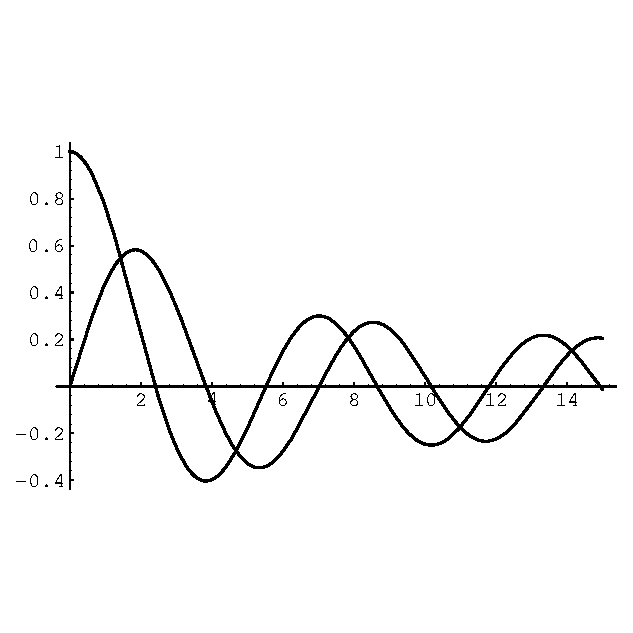
\includegraphics[width=0.49\textwidth]{ode/bessel/bessj12}
    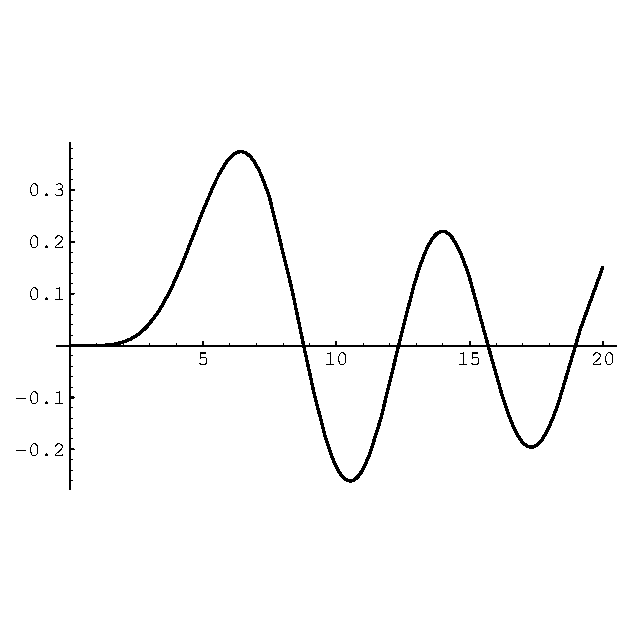
\includegraphics[width=0.49\textwidth]{ode/bessel/besselj5}
  \end{center}
  \caption{Bessel functions of the first kind.}
  \label{besselj125}
\end{figure}









%%--------------------------------------------------------------------------
\subsection{Series Expansion of the Bessel Function}



We expand $\exp(-z^2/4t)$ in the integral expression for $J_n$.
\begin{align*}
  J_n(z)  
  &= \frac{1}{\imath 2 \pi} \left(\frac{z}{2}\right)^n \oint t^{-n-1} \e^{t-z^2/4t}\,\dd t 
  \\
  &= \frac{1}{\imath 2 \pi} \left(\frac{z}{2}\right)^n \oint t^{-n-1}
  \e^t \left( \sum_{m = 0}^\infty \left(\frac{-z^2}{4 t}\right)^m
    \frac{1}{m!} \right)\,\dd t
\end{align*}
For the path of integration, we are free to choose any contour that encloses
the origin.  Consider the circular path on $|t| = 1$.  Since the integral
is uniformly convergent, we can interchange the order of integration and 
summation.
\[ 
J_n(z) = \frac{1}{\imath 2 \pi} \left(\frac{z}{2}\right)^n \sum_{m = 0}^\infty 
\frac{(-1)^m z^{2m}}{2^{2m} m!} \oint t^{-n-m-1} \e^t\,\dd t 
\]

Let $n$ be a non-negative integer.
\begin{align*}
  \frac{1}{\imath 2 \pi} \oint t^{-n-m-1} \e^t\,\dd t
  &= \lim_{z \to 0} \left( \frac{1}{(n + m)!} \frac{\dd^{n+m}}{\dd z^{n+m}}
    (\e^z) \right) 
  \\
  &= \frac{1}{(n+m)!}
\end{align*}
We have the series expansion
\[ 
\boxed{ 
  J_n(z) = \sum_{m = 0}^\infty \frac{(-1)^m}{m! (n+m)!} \left( 
    \frac{z}{2}\right)^{n+2m} \quad \mathrm{for}\ n \geq 0. 
  } 
\]

Now consider $J_{-n}(z)$, ($n$ positive).
\[ 
J_{-n}(z) = \frac{1}{\imath 2 \pi} \left( \frac{z}{2} \right)^{-n} \sum_{m = 1}^\infty
\frac{ (-1)^m z^{2m}}{2^{2m} m!} \oint t^{n-m-1} \e^t\,\dd t 
\]
For $m \geq n$, the integrand has a pole of order $m - n + 1$ at the origin.
\[ 
\frac{1}{\imath 2 \pi} \oint t^{n-m-1}\e^t\,\dd t = 
\begin{cases}
  \frac{1}{(m - n)!} \quad &\mathrm{for}\ m \geq n \\
  0 \quad &\mathrm{for}\ m < n
\end{cases} \]
The expression for $J_{-n}$ is then
\begin{align*}
  J_{-n}(z)
  &= \sum_{m=n}^\infty \frac{(-1)^m}{m! (m - n)!} \left( \frac{z}{2} \right)^{-n+2m} 
  \\
  &= \sum_{m = 0}^\infty \frac{(-1)^{m + n}}{(m + n)! m!} \left( \frac{z}{2} \right)^{n + 2 m} 
  \\
  &= (-1)^n J_n(z).
\end{align*}
Thus we have that 
\[ 
\boxed{
  J_{-n}(z) = (-1)^n J_n(z) \quad \mathrm{for integer}\ n.
  } 
\]








%%--------------------------------------------------------------------------
\subsection{Bessel Functions of Non-Integer Order}

The generalization of the factorial function is the Gamma function.
For integer values of $n$, $n! = \Gamma(n+1)$.  The Gamma function is defined
for all complex-valued arguments.  Thus one would guess that if the 
Bessel function of the first kind were defined for non-integer order, it
would have the definition,
\[ 
J_\nu(z) = \sum_{m = 0}^\infty \frac{(-1)^m}{m! \Gamma(\nu+m+1)} \left( \frac{z}{2} \right)^{\nu+2m}.
\]

\paragraph{The Integrand for Non-Integer $\mathbf{\boldsymbol{\nu}}$.}
Recall the definition of the Bessel function
\[ 
J_\nu(z) = \frac{1}{\imath 2 \pi} \left( \frac{z}{2} \right)^\nu \oint t^{-\nu-1}
\e^{t - z^2/4t}\,\dd t.
\]
When $\nu$ is an integer, the integrand is single valued.  Thus if you start
at any point and follow any path around the origin, the integrand will
return to its original value.  This property was the key to $J_n$ satisfying
Bessel's equation.  If $\nu$ is not an integer, then this property does not
hold for arbitrary paths around the origin.


\paragraph{A New Contour.}
First, since the integrand is multiple-valued, we need to define what 
branch of the function we are talking about.  We will take the principal
value of the integrand and introduce a branch cut on the negative real
axis.  Let $C$ be a contour that starts at $z = -\infty$ below the branch
cut, circles the origin, and returns to the point $z = -\infty$ above the 
branch cut.  This contour is shown in Figure~\ref{fig_cont_int}.

\begin{figure}[h!]
  \begin{center}
    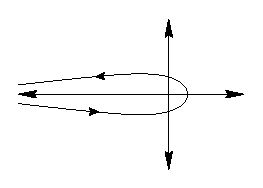
\includegraphics[width=0.25\textwidth]{ode/gamma/fig_hank_cont}
  \end{center}

  \caption{The contour of integration.}
  \label{fig_cont_int}
\end{figure}



Thus we define
\[ 
\boxed{
  J_\nu(z) = \frac{1}{\imath 2 \pi} \left( \frac{z}{2} \right)^\nu \oint_C 
  t^{-\nu-1} \e^{t - z^2/4t}\,\dd t.
  } 
\]

\paragraph{Bessel's Equation.}
Substituting $J_\nu(z)$ into Bessel's equation yields
\[ 
J_\nu'' + \frac{1}{z} J_\nu' + \left(1 - \frac{\nu^2}{z^2} \right) J_\nu = 
\frac{1}{\imath 2 \pi} \left(\frac{z}{2}\right)^\nu \oint_C \frac{\dd}{\dd t}
\left(t^{-\nu-1}\e^{t-z^2/4t} \right) \,\dd t.
\]
Since $t^{-\nu-1}\e^{t-z^2/4t}$ is analytic in $0 < |z| < \infty$ and 
$|\arg(z)| < \pi$, and it vanishes at $z = - \infty$, the integral is zero.  
Thus the Bessel function of the first kind satisfies Bessel's 
equation for all complex orders.



\paragraph{Series Expansion.}
Because of the $\e^t$ factor in the integrand, the integral defining $J_\nu$
converges uniformly.  Expanding $\e^{-z^2/4t}$ in a Taylor series yields
\[ 
J_\nu(z) = \frac{1}{\imath 2 \pi} \left(\frac{z}{2}\right)^\nu \sum_{m = 0}^\infty
\frac{(-1)^m z^{2m}}{2^{2m} m!} \oint_C t^{-\nu-m-1} \e^t\,\dd t 
\]
Since
\[ 
\frac{1}{\Gamma(\alpha)} = \frac{1}{\imath 2 \pi} \oint_C t^{-\alpha-1} \e^t\,\dd t,
\]
we have the series expansion of the Bessel function
\[ 
\boxed{
J_\nu(z) = \sum_{m = 0}^\infty \frac{(-1)^m}{m! \Gamma(\nu+m+1)} 
  \left( \frac{z}{2} \right)^{\nu+2m}.
  }
\]




\paragraph{Linear Independence.}
We use Abel's formula to compute the Wronskian of Bessel's equation.
\[ 
W(z) = \exp\left(-\int^z \frac{1}{\zeta}\,\dd \zeta \right)
= \e^{-\log z} = \frac{1}{z}
\]
Thus to within a function of $\nu$, the Wronskian of any two solutions is $1/z$.
For any given 
$\nu$, there are two linearly independent solutions.
Note that Bessel's equation is unchanged under the transformation $\nu \to 
-\nu$. Thus both $J_\nu$ and $J_{-\nu}$ satisfy Bessel's equation.  
Now we must determine if they are linearly independent.  We have already
shown that for integer values of $\nu$ they are not independent.
($J_{-n} = (-1)^n J_n$.)  Assume that $\nu$ is not an integer.
We compute the Wronskian of $J_\nu$ and $J_{-\nu}$.
\begin{align*}
  W[J_\nu, J_{-\nu}]
  &= \begin{vmatrix}
    J_\nu   &       J_{-\nu}        \\
    J_\nu'  &       J_{-\nu}'
  \end{vmatrix} 
  \\
  &= J_\nu J_{-\nu}' - J_{-\nu} J_\nu' 
  \\
  \intertext{We substitute in the expansion for $J_\nu$}
  &= \left( \sum_{m = 0}^\infty \frac{(-1)^m}{m! \Gamma(\nu+m+1)} 
    \left(\frac{z}{2}\right)^{\nu+2m} \right)
  \left( \sum_{n = 0}^\infty \frac{(-1)^n (-\nu+2n)}{n! \Gamma(-\nu+n+1)2}
    \left(\frac{z}{2}\right)^{-\nu+2n-1}\right) 
  \\
  &\qquad - 
  \left( \sum_{m = 0}^\infty \frac{(-1)^m}{m! \Gamma(-\nu+m+1)} 
    \left(\frac{z}{2}\right)^{-\nu+2m} \right)
  \left( \sum_{n = 0}^\infty \frac{(-1)^n (\nu+2n)}{n! \Gamma(\nu+n+1)2}
    \left(\frac{z}{2}\right)^{\nu+2n-1}\right)
  \\ 
  \intertext{Since the Wronskian is a function of $\nu$ times $1/z$ the 
    coefficients of all of the powers of $z$ except $1/z$ must vanish.}
  &= \frac{-\nu}{z \Gamma(\nu+1) \Gamma(-\nu+1)}
  - \frac{\nu}{z \Gamma(-\nu+1) \Gamma(\nu+1)} 
  \\
  &= - \frac{2}{z \Gamma(\nu) \Gamma(1-\nu)} 
  \\
  \intertext{Using an identity for the Gamma function simplifies this 
    expression.}
  &= -\frac{2}{\pi z} \sin(\pi \nu)
\end{align*}
Since the Wronskian is nonzero for non-integer $\nu$, $J_\nu$ and $J_{-\nu}$
are independent functions when $\nu$ is not an integer.  In this case, the 
general solution of Bessel's equation is $a J_\nu + b J_{-\nu}$.  








%%-----------------------------------------------------------------------------
\subsection{Recursion Formulas}

In showing that $J_\nu$ satisfies Bessel's equation for arbitrary complex 
$\nu$, we obtained 
\begin{gather*}
  \oint_C \frac{\dd}{\dd t} \left( t^{-\nu} \e^{t - z^2/4t} \right)\,\dd t = 0. 
  \\
  \intertext{Expanding the integral,}
  \oint_C \left( t^{-\nu} + \frac{z^2}{4} t^{-\nu-2} -\nu t^{-\nu-1} \right)
  \e^{t-z^2/4t}\,\dd t = 0. 
  \\
  \frac{1}{\imath 2 \pi} \left( \frac{z}{2} \right)^\nu 
  \oint_C \left( t^{-\nu} + \frac{z^2}{4} t^{-\nu-2} -\nu t^{-\nu-1} 
  \right) \e^{t-z^2/4t}\,\dd t = 0. 
  \\
  \intertext{Since $J_\nu(z) = \frac{1}{\imath 2 \pi} (z/2)^\nu \oint_C t^{-\nu-1} 
    \e^{t-z^2/4t}\,\dd t$,}
  \left[\left(\frac{2}{z}\right)^{-1} J_{\nu-1} + \left(\frac{2}{z}
    \right) \frac{z^2}{4} J_{\nu+1} - \nu J_\nu \right] = 0. 
  \\
  \boxed{
    J_{\nu-1} + J_{\nu+1} = \frac{2 \nu}{z} J_\nu 
    }
\end{gather*}

Differentiating the integral expression for $J_\nu$, 
\begin{gather*}
  J_\nu'(z) = \frac{1}{\imath 2 \pi} \frac{\nu z^{\nu-1}}{2^\nu} \oint_C t^{-\nu-1}\e^{t-z^2/4t}\,\dd t 
  + \frac{1}{\imath 2 \pi} \left(\frac{z}{2}\right)^\nu \oint_C 
  t^{-\nu-1} \left(-\frac{z}{2 t}\right) \e^{t-z^2/4t}\,\dd t 
  \\
  J_\nu'(z)= \frac{\nu}{z} \frac{1}{\imath 2 \pi} \left(\frac{z}{2}\right)^\nu 
  \oint_C t^{-\nu-1}\e^{t-z^2/4t} \,\dd t - 
  \frac{1}{\imath 2 \pi} \left(\frac{z}{2}\right)^{\nu+1} 
  \oint_C t^{-\nu-2}\e^{t-z^2/4t} \,\dd t 
  \\
  \boxed{ 
    J_\nu' = \frac{\nu}{z} J_\nu - J_{\nu+1} 
    }
\end{gather*}


From the two relations we have derived you can show that
\[
\boxed{
  J_\nu' = \frac{1}{2} (J_{\nu-1} + J_{\nu+1})
  } 
\qquad \mathrm{and} \qquad 
\boxed{
  J_\nu' = J_{\nu-1} - \frac{\nu}{z} J_\nu.
  }
\]





\begin{Result}
  The Bessel function of the first kind, $J_\nu(z)$,  is defined,
  \[ 
  J_\nu(z) = \frac{1}{\imath 2 \pi} \left(\frac{z}{2} \right)^\nu \oint_C t^{-\nu-1}
  \e^{t - z^2/4t}\,\dd t. 
  \]
  The Bessel function has the expansion,
  \[ 
  J_\nu(z) = \sum_{m = 0}^\infty \frac{(-1)^m}{m! \Gamma(\nu+m+1)} \left( \frac{z}{2} \right)^{\nu+2m}. 
  \]
  The asymptotic behavior for large argument is
  \[
  J_\nu(z) \sim \sqrt{ \frac{2}{\pi z} } \left(
    \cos \left( z - \frac{\nu \pi}{2} - \frac{\pi}{4} \right) 
    + \e^{|\Im(z)|} \mathcal{O}\left( |z|^{-1} \right) \right)
  \quad \mathrm{as}\ |z| \to \infty, ~ |\arg(z)| < \pi.
  \]
  The Wronskian of $J_\nu(z)$ and $J_{-\nu}(z)$ is
  \[ 
  W(z) = -\frac{2}{\pi z} \sin(\pi \nu). 
  \]
  Thus $J_\nu(z)$ and $J_{-\nu}(z)$ are independent when $\nu$ is not 
  an integer.
  The Bessel functions satisfy the recursion relations,
  \begin{alignat*}{2}
    &J_{\nu-1} + J_{\nu+1} = \frac{2\nu}{z} J_\nu &\qquad
    &J_\nu' = \frac{\nu}{z} J_\nu - J_{\nu+1} \\
    &J_\nu' = \frac{1}{2} (J_{\nu-1} - J_{\nu+1}) &\qquad
    &J_\nu' = J_{\nu-1} - \frac{\nu}{z} J_\nu.
  \end{alignat*}
\end{Result}


















%%---------------------------------------------------------------------------
\subsection{Bessel Functions of Half-Integer Order}

Consider $J_{1/2}(z)$.  Start with the series expansion
\begin{align*}
  J_{1/2}(z)
  &= \sum_{m = 0}^\infty \frac{(-1)^m}{m! \Gamma(1/2 + m + 1)} \left( \frac{z}{2}
  \right)^{1/2 + 2m}. 
  \\
  \intertext{Use the identity $\Gamma(n+1/2) = \frac{(1)(3)\cdots(2n-1)}{2^n}
    \sqrt{\pi}$.}
  &= \sum_{m = 0}^\infty \frac{(-1)^m 2^{m+1}}{m! (1)(3)\cdots(2m+1) \sqrt{\pi}}
  \left(\frac{z}{2}\right)^{1/2+2m} 
  \\
  &= \sum_{m = 0}^\infty \frac{(-1)^m 2^{m+1}}{(2)(4)\cdots(2m) \cdot (1)(3)\cdots
    (2m+1) \sqrt{\pi}} \left(\frac{1}{2} \right)^{1/2 + m}
  z^{1/2 + 2m} 
  \\
  &= \left( \frac{2}{\pi z} \right)^{1/2} \sum_{m = 0}^\infty \frac{(-1)^m}
  {(2m+1)!} z^{2m+1} 
  \\
  \intertext{We recognize the sum as the Taylor series expansion of $\sin z$.}
  &= \left( \frac{2}{\pi z} \right)^{1/2} \sin z
\end{align*}

Using the recurrence relations,
\[ 
J_{\nu+1} = \frac{\nu}{z} J_\nu - J_\nu' \quad \mathrm{and} \quad
J_{\nu-1} = \frac{\nu}{z} J_\nu + J_\nu', 
\]
we can find $J_{n+1/2}$ for any integer $n$.




\begin{Example}
  To find $J_{3/2}(z)$,
  \begin{align*}
    J_{3/2}(z)
    &= \frac{1/2}{z} J_{1/2}(z) - J_{1/2}'(z) 
    \\
    &= \frac{1/2}{z} \left( \frac{2}{\pi} \right)^{1/2} z^{-1/2} \sin z
    - \left(-\frac{1}{2}\right) \left(\frac{2}{\pi}\right)^{1/2}
    z^{-3/2} \sin z - \left(\frac{2}{\pi}\right)^{1/2} z^{-1/2}
    \cos z 
    \\
    &= 2^{-1/2} \pi^{-1/2} z^{-3/2} \sin z
    + 2^{-1/2} \pi^{-1/2} z^{-3/2} \sin z
    - 2^{-1/2} \pi^{-1/2} \cos z 
    \\
    &= \left(\frac{2}{\pi}\right)^{1/2} z^{-3/2} \sin z
    - \left(\frac{2}{\pi}\right)^{1/2} z^{-1/2} \cos z 
    \\
    &= \left(\frac{2}{\pi}\right)^{1/2} \left( z^{-3/2} \sin z
      - z^{-1/2} \cos z \right).
  \end{align*}
  You can show that 
  \[ 
  J_{-1/2}(z) = \left( \frac{2}{\pi z} \right)^{1/2} \cos z. 
  \]
\end{Example}


Note that at a first glance it appears that $J_{3/2} \sim z^{-1/2}$ as 
$z \to 0$.  However, if you expand the sine and cosine you will see that the
$z^{-1/2}$ and $z^{1/2}$ terms vanish and thus $J_{3/2}(z) \sim z^{3/2}$
as $z \to 0$ as we showed previously.



Recall that we showed the asymptotic behavior as $x \to +\infty$
of Bessel functions to be linear combinations of
\[ 
x^{-1/2} \sin(x + U_1(x)) \quad \mathrm{and} \quad 
x^{-1/2} \cos(x + U_2(x)) 
\]
where $U_1, U_2 \to 0$ as $x \to +\infty$.






%%===========================================================================
\section{Neumann Expansions}


Consider expanding an analytic function in a series of Bessel functions of
the form
\[ 
f(z) = \sum_{n = 0}^\infty a_n J_n(z). 
\]
If $f(z)$ is analytic in the disk $|z| \leq r$ then we can write
\[ 
f(z) = \frac{1}{\imath 2 \pi} \oint \frac{f(\zeta)}{\zeta - z}\,\dd \zeta ,
\]
where the path of integration is $|\zeta| = r$ and $|z| < r$.  
If we were able to expand the function $\frac{1}{\zeta-z}$ in a series of 
Bessel functions, then we could interchange the order of summation and 
integration to get a Bessel series expansion of $f(z)$.  



\paragraph{The Expansion of $\mathbf{1 \boldsymbol{/} \boldsymbol{(} 
\boldsymbol{\zeta} - z \boldsymbol{)} }$.}
Assume that $\frac{1}{\zeta-z}$ has the uniformly convergent expansion
\[ 
\frac{1}{\zeta-z} = c_0(\zeta) J_0(z) + 2 \sum_{n = 1}^\infty c_n(\zeta) J_n(z), 
\]
where each $c_n(\zeta)$ is analytic.
Note that
\[ 
\left( \frac{\partial}{\partial \zeta} + \frac{\partial}{\partial z} \right) \frac{1}{\zeta-z}
= \frac{-1}{(\zeta-z)^2} + \frac{1}{(\zeta-z)^2} = 0. 
\]
Thus we have
\begin{align*}
  \left( \frac{\partial}{\partial \zeta} + \frac{\partial}{\partial z} \right) \left[ c_0(\zeta) J_0(z)
    + 2 \sum_{n = 1}^\infty c_n(\zeta) J_n(z) \right] &= 0 
  \\
  \left[ c_0' J_0 + 2 \sum_{n = 1}^\infty c_n' J_n \right] + \left[ c_0 J_0' + 
    2 \sum_{n = 1}^\infty c_n J_n' \right] &= 0. 
  \\
  \intertext{Using the identity $2J_n' = J_{n-1} - J_{n+1}$,}
  \left[ c_0' J_0 + 2 \sum_{n = 1}^\infty c_n' J_n \right] + \left[ c_0 (-J_1) + 
    \sum_{n = 1}^\infty c_n (J_{n-1} - J_{n+1}) \right] &= 0. 
  \\
  \intertext{Collecting coefficients of $J_n$, }
  (c_0' + c_1) J_0 + \sum_{n = 1}^\infty (2c_n' + c_{n+1} - c_{n-1})J_n &= 0.
\end{align*}
Equating the coefficients of $J_n$, we see that the $c_n$ are given by the 
relations,
\[ 
c_1 = -c_0', \quad \mathrm{and} \quad 
c_{n+1} = c_{n-1} - 2 c_n'. 
\]


We can evaluate $c_0(\zeta)$.  Setting $z = 0$, 
\begin{align*}
  \frac{1}{\zeta} &= c_0(\zeta) J_0(0) + 2 \sum_{n = 1}^\infty c_n(\zeta) J_n(0) 
  \\
  \frac{1}{\zeta} &= c_0(\zeta).
\end{align*}

Using the recurrence relations we can calculate the $c_n$'s.  The first few
are:
\begin{align*}
  c_1 &= - \frac{-1}{\zeta^2} = \frac{1}{\zeta^2} 
  \\
  c_2 &= \frac{1}{\zeta} - 2 \frac{-2}{\zeta^3} = \frac{1}{\zeta} 
  + \frac{4}{\zeta^3} 
  \\
  c_3 &= \frac{1}{\zeta^2} - 2 \left( \frac{-1}{\zeta^2} - \frac{12}{\zeta^4}
  \right) = \frac{3}{\zeta^2} + \frac{24}{\zeta^4}.
\end{align*}
We see that $c_n$ is a polynomial of degree $n+1$ in $1/\zeta$. One can show
that
\[ c_n(\zeta) = \begin{cases}
  \frac{2^{n-1} n!}{\zeta^{n+1}} \left( 1 + \frac{\zeta^2}{2(2n-2)}
    + \frac{\zeta^4}{2\cdot 4 \cdot (2n-2)(2n-4)} + \cdots + 
    \frac{\zeta^n}{2\cdot 4 \cdots n \cdot (2n-2)\cdots (2n-n)}
  \right)
  \quad &\mathrm{for even}\ n 
  \\
  \frac{2^{n-1} n!}{\zeta^{n+1}} \left( 1 + \frac{\zeta^2}{2(2n-2)}
    + \frac{\zeta^4}{2\cdot 4 \cdot (2n-2)(2n-4)} + \cdots + 
    \frac{\zeta^{n-1}}
    {2\cdot 4 \cdots (n-1) \cdot (2n-2)\cdots (2n-(n-1))}\right)
  \quad &\mathrm{for odd}\ n 
\end{cases}
\]



\paragraph{Uniform Convergence of the Series.}
We assumed before that the series expansion of $\frac{1}{\zeta-z}$ is
uniformly convergent.  The behavior of $c_n$ and $J_n$ are
\[ 
c_n(\zeta) = \frac{2^{n-1} n!}{\zeta^{n+1}} + O(\zeta^{-n}), \qquad
J_n(z) = \frac{z^n}{2^n n!} + O(z^{n+1}). 
\]
This gives us
\[ 
c_n(\zeta)J_n(z) = \frac{1}{2\zeta} \left(\frac{z}{\zeta}\right)^n
+ \mathcal{O}\left( \frac{1}{\zeta} \left( \frac{z}{\zeta}\right)^{n+1}\right).
\]
If $\left| \frac{z}{\zeta}\right| = \rho < 1$ we can bound the series
with the geometric series $\sum \rho^n$.  Thus the series is uniformly 
convergent.


\paragraph{Neumann Expansion of an Analytic Function.}
Let $f(z)$ be a function that is analytic in the disk $|z| \leq r$.  
Consider $|z| < r$ and the path of integration along $|\zeta| = r$.  
Cauchy's integral formula tells us that
\begin{align*}
  f(z)    
  &= \frac{1}{\imath 2 \pi} \oint \frac{f(\zeta)}{\zeta-z}\,\dd \zeta. 
  \\
  \intertext{Substituting the expansion for $\frac{1}{\zeta-z}$,}
  &= \frac{1}{\imath 2 \pi} \oint f(\zeta) \left( c_o(\zeta) J_0(z) + 
    2 \sum_{n = 1}^\infty c_n(\zeta) J_n(z) \right)\,\dd \zeta 
  \\
  &= J_0(z) \frac{1}{\imath 2 \pi} \oint \frac{f(\zeta)}{\zeta}\,\dd \zeta + 
  \sum_{n = 1}^\infty \frac{J_n(z)}{\imath \pi} \oint c_n(\zeta) f(\zeta)\,\dd \zeta 
  \\
  &= J_0(z) f(0) + \sum_{n = 1}^\infty \frac{J_n(z)}{\imath \pi} \oint c_n(\zeta) f(\zeta)\,\dd \zeta.
\end{align*}





\begin{Result}
  let $f(z)$ be analytic in the disk, $|z| \leq r$.  Consider $|z| < r$ and the
  path of integration along $|\zeta| = r$.  $f(z)$ has the Bessel function
  series expansion
  \[ 
  f(z) = J_0(z) f(0) + \sum_{n = 1}^\infty \frac{J_n(z)}{\imath \pi} \oint c_n(\zeta) f(\zeta)\,\dd \zeta, 
  \]
  where the $c_n$ satisfy
  \[ 
  \frac{1}{\zeta - z} = c_0(\zeta) J_0(z) + 2 \sum_{n = 1}^\infty c_n(\zeta) J_n(z). 
  \]
\end{Result}











%%============================================================================
\section{Bessel Functions of the Second Kind}
\index{Bessel functions!second kind}
\index{Weber's function}


When $\nu$ is an integer, $J_\nu$ and $J_{-\nu}$ are not linearly 
independent.  In order to find an second linearly independent solution,
we define the Bessel function of the second kind, (also called 
\textbf{Weber's function}),
\[ 
Y_\nu
= \begin{cases}
  \frac{J_\nu(z) \cos(\nu \pi) 
    - J_{-\nu}(z)}{\sin(\nu \pi)} 
  \quad &\mathrm{when}\ \nu\ \mathrm{is not an integer} \\
  \lim_{\mu \to \nu} \frac{J_\mu(z) \cos(\mu \pi) 
    - J_{-\mu}(z)}{\sin(\mu \pi)} 
  \quad &\mathrm{when}\ \nu\ \mathrm{is an integer}.
\end{cases}
\]
$J_\nu$ and $Y_\nu$ are linearly independent for all $\nu$.

In Figure~\ref{bessely} $Y_0$ and $Y_1$ are plotted in solid and dashed lines,
respectively.


\begin{figure}[h!]
  \begin{center}
    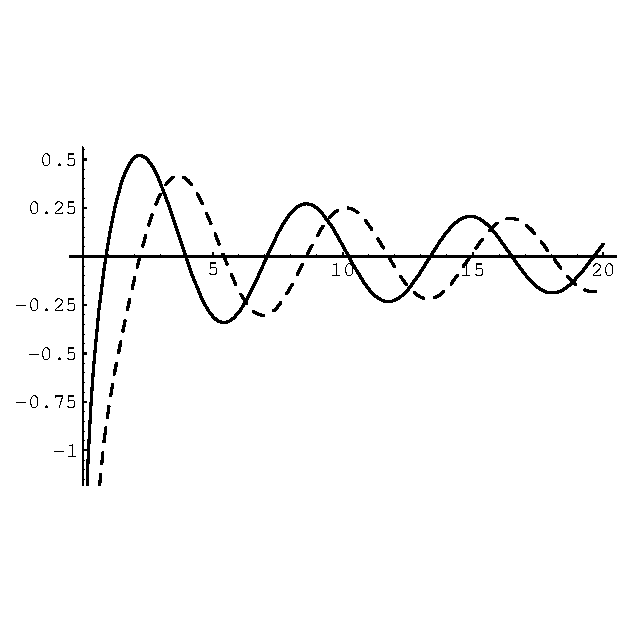
\includegraphics[width=0.5\textwidth]{ode/bessel/bessely}
  \end{center}
  \caption{Bessel functions of the second kind.}
  \label{bessely}
\end{figure}



\begin{Result}
  The Bessel function of the second kind, $Y_\nu(z)$,  is defined,
  \[ Y_\nu
  = \begin{cases}
    \frac{J_\nu(z) \cos(\nu \pi) 
      - J_{-\nu}(z)}{\sin(\nu \pi)} 
    \quad &\mathrm{when}\ \nu\ \mathrm{is not an integer} \\
    \lim_{\mu \to \nu} \frac{J_\mu(z) \cos(\mu \pi) 
      - J_{-\mu}(z)}{\sin(\mu \pi)} 
    \quad &\mathrm{when}\ \nu\ \mathrm{is an integer}.
  \end{cases}
  \]
  The Wronskian of $J_\nu(z)$ and $Y_\nu(z)$ is
  \[ W[J_\nu, Y_\nu] = \frac{2}{\pi z}. \]
  Thus $J_\nu(z)$ and $Y_\nu(z)$ are independent for all $\nu$.
  The Bessel functions of the second kind satisfy the recursion relations,
  \begin{alignat*}{2}
    &Y_{\nu-1} + Y_{\nu+1} = \frac{2\nu}{z} Y_\nu &\qquad
    &Y_\nu' = \frac{\nu}{z} Y_\nu - Y_{\nu+1} 
    \\
    &Y_\nu' = \frac{1}{2} (Y_{\nu-1} - Y_{\nu+1}) &\qquad
    &Y_\nu' = Y_{\nu-1} - \frac{\nu}{z} Y_\nu.
  \end{alignat*}
\end{Result}



















%%=============================================================================
\section{Hankel Functions}


Another set of solutions to Bessel's equation is the Hankel functions,
\begin{align*}
  H_\nu^{(1)}(z) &= J_\nu(z) + \imath Y_\nu(z), 
  \\
  H_\nu^{(2)}(z) &= J_\nu(z) - \imath Y_\nu(z) 
\end{align*}



\begin{Result}
  The Hankel functions are defined
  \begin{align*}
    H_\nu^{(1)}(z) &= J_\nu(z) + \imath Y_\nu(z), 
    \\
    H_\nu^{(2)}(z) &= J_\nu(z) - \imath Y_\nu(z) 
  \end{align*}
  The Wronskian of $H_\nu^{(1)}(z)$ and $H_\nu^{(2)}(z)$ is
  \[ 
  W[H_\nu^{(1)}, H_\nu^{(2)}] = - \frac{\imath 4}{\pi z}. 
  \]
  The Hankel functions are independent for all $\nu$.
  The Hankel functions satisfy the same recurrence relations as the other
  Bessel functions.
\end{Result}









%%============================================================================
\section{The Modified Bessel Equation}





The modified Bessel equation is
\[ 
w'' + \frac{1}{z} w' - \left(1 + \frac{\nu^2}{z^2} \right) w = 0. 
\]
This equation is identical to the Bessel equation except for a sign change
in the last term.  If we make the change of variables $\xi = \imath z$, 
$u(\xi) = w(z)$ we obtain the equation
\begin{gather*}
  -u'' - \frac{1}{\xi} u' - \left(1 - \frac{\nu^2}{\xi^2} \right) u = 0 
  \\
  u'' + \frac{1}{\xi} u' + \left(1 - \frac{\nu^2}{\xi^2} \right) u = 0.
\end{gather*}
This is the Bessel equation.  Thus $J_\nu(\imath z)$ is a solution to the modified
Bessel equation.  This motivates us to define the modified Bessel function
of the first kind
\[ 
I_\nu(z) = \imath^{-\nu} J_\nu(\imath z). 
\]
Since $J_\nu$ and $J_{-\nu}$ are linearly independent solutions when $\nu$ is not
an integer, $I_\nu$ and $I_{-\nu}$ are linearly independent solutions 
to the modified Bessel equation when $\nu$ is not an integer.

The Taylor series expansion of $I_\nu(z)$ about $z = 0$ is
\begin{align*}
  I_\nu(z)
  &= \imath^{-\nu} J_\nu(\imath z) 
  \\
  &= \imath^{-\nu} \sum_{m = 0}^\infty \frac{(-1)^m}{m! \Gamma(\nu+m+1)} \left( \frac{\imath z}{2} \right)^{\nu+2m} 
  \\
  &= \imath^{-\nu} \sum_{m = 0}^\infty \frac{(-1)^m \imath^\nu \imath^{2m}}{m! \Gamma(\nu+m+1)} 
  \left( \frac{z}{2} \right)^{\nu+2m} 
  \\
  &= \sum_{m = 0}^\infty \frac{1}{m! \Gamma(\nu + m + 1)} \left( \frac{z}{2} \right)^{\nu + 2 m} 
\end{align*}



\paragraph{Modified Bessel Functions of the Second Kind.}
In order to have a second linearly independent solution when $\nu$ is an 
integer, we define the modified Bessel function of the second kind
\[ 
K_\nu(z) = 
\begin{cases}
  \frac{\pi}{2} \frac{I_{-\nu} - I_\nu}{\sin(\nu \pi)} 
  \quad &\mathrm{when}\ \nu\ \mathrm{is not an integer},
  \\
  \lim_{\mu \to \nu} \frac{\pi}{2} \frac{I_{-\mu} - I_\mu}{\sin(\mu \pi)} 
  \quad &\mathrm{when}\ \nu\ \mathrm{is an integer}.
\end{cases}
\]
$I_\nu$ and $K_\nu$ are linearly independent for all $\nu$.
In Figure~\ref{besselik} $I_0$ and $K_0$ are plotted in solid and dashed lines,
respectively.  


\begin{figure}[h!]
  \begin{center}
    \includegraphics[width=0.5\textwidth]{ode/bessel/besselik}
  \end{center}
  \caption{Modified Bessel functions.}
  \label{besselik}
\end{figure}








\begin{Result}
  The modified Bessel functions of the first and second kind, $I_\nu(z)$ and 
  $K_\nu(z)$, are defined,
  \[ 
  I_\nu(z) = \imath^{-\nu} J_\nu(\imath z). 
  \]
  \[ K_\nu(z) = 
  \begin{cases}
    \frac{\pi}{2} \frac{I_{-\nu} - I_\nu}{\sin(\nu \pi)} 
    \quad &\mathrm{when}\ \nu\ \mathrm{is not an integer}, 
    \\
    \lim_{\mu \to \nu} \frac{\pi}{2} \frac{I_{-\mu} - I_\mu}{\sin(\mu \pi)} 
    \quad &\mathrm{when}\ \nu\ \mathrm{is an integer}.
  \end{cases}
  \]
  The modified Bessel function of the first kind has the expansion,
  \[
  I_\nu(z) = \sum_{m = 0}^\infty \frac{1}{m! \Gamma(\nu + m + 1)} \left( \frac{z}{2} \right)^{\nu+2m} 
  \]
  The Wronskian of $I_\nu(z)$ and $I_{-\nu}(z)$ is
  \[
  W[I_\nu,I_{-\nu}] = - \frac{2}{\pi z} \sin(\pi \nu).
  \]
  $I_\nu(z)$ and $I_{-\nu}(z)$ are linearly independent when $\nu$ is not an 
  integer.
  The Wronskian of $I_\nu(z)$ and $K_\nu(z)$ is
  \[
  W[I_\nu,K_\nu] = - \frac{1}{z}.
  \]
  $I_\nu(z)$ and $K_\nu(z)$ are independent for all $\nu$.
  The modified Bessel functions satisfy the recursion relations,
  \begin{alignat*}{2}
    &A_{\nu-1} - A_{\nu+1} = \frac{2\nu}{z} A_\nu &\qquad
    &A_\nu' = A_{\nu+1} + \frac{\nu}{z} A_\nu 
    \\
    &A_\nu' = \frac{1}{2} (A_{\nu-1} + A_{\nu+1}) &\qquad
    &A_\nu' = A_{\nu-1} - \frac{\nu}{z} A_\nu.
  \end{alignat*}
  where $A$ stands for either $I$ or $K$.
\end{Result}

















\raggedbottom
%%============================================================================
\exercises{
\pagebreak
\flushbottom
\section{Exercises}






%% Frobenius solution
\begin{Exercise}
  Consider Bessel's equation
  \[
  z^2 y''(z) + z y'(z) + \left( z^2 - \nu^2 \right) y = 0
  \]
  where $\nu \geq 0$.  Find the Frobenius series solution that is asymptotic
  to $t^\nu$ as $t \to 0$.  By multiplying this solution by a constant, 
  define the solution
  \[
  J_\nu(z) = \sum_{k = 1}^\infty \frac{(-1)^k}{k! \Gamma(k + \nu + 1)} 
  \left( \frac{z}{2} \right)^{2k + \nu}.
  \]
  This is called the Bessel function of the first kind and order $\nu$.
  Clearly $J_{-\nu}(z)$ is defined and is linearly independent to $J_\nu(z)$
  if $\nu$ is not an integer.  What happens when $\nu$ is an integer?
\end{Exercise}




%% CONTINUE:
%% Check this
%% Bessel's equation for integer n
\begin{Exercise}
  Consider Bessel's equation for integer $n$,
  \[
  z^2 y'' + z y' + \left( z^2 - n^2 \right) y = 0.
  \]
  Using the kernel
  \[
  K(z,t) = \e^{ \frac{1}{2} z \left( t - \frac{1}{t} \right) },
  \]
  find two solutions of Bessel's equation.  (For $n = 0$ you will find only
  one solution.)  Are the two solutions linearly independent?  Define
  the Bessel function of the first kind and order $n$,
  \[
  J_n(z) = \frac{1}{\imath 2 \pi} \oint_C t^{-n-1} \e^{ \frac{1}{2} z (t - 1/t) } \,\dd t,
  \]
  where $C$ is a simple, closed contour about the origin.
  Verify that
  \[
  \e^{ \frac{1}{2} z (t - 1/t) } = \sum_{n = -\infty}^\infty J_n(z) t^n.
  \]
  This is the \textit{generating function} for the Bessel functions.
\end{Exercise}




%% Use generating function to show that $J_n$ satisfies Bessel's equation
\begin{Exercise}
  Use the generating function 
  \[
  \e^{ \frac{1}{2} z (t - 1/t) } = \sum_{n = -\infty}^\infty J_n(z) t^n
  \]
  to show that $J_n$ satisfies Bessel's equation
  \[
  z^2 y'' + z y' + \left( z^2 - n^2 \right) y = 0.
  \]
\end{Exercise}




%%1111111111111111111111111111111111111111111111111111111111111111111111111111
\begin{Exercise}
  Using
  \[ 
  J_{n-1} + J_{n+1} = \frac{2 n}{z} J_n \quad \mathrm{and} \quad
  J_n' = \frac{n}{z} J_n - J_{n+1},
  \]
  show that
  \[ 
  J_n' = \frac{1}{2}(J_{n-1} - J_{n+1}) \quad \mathrm{and} \quad
  J_n' = J_{n-1} - \frac{n}{z} J_n.
  \]
\end{Exercise}



%%22222222222222222222222222222222222222222222222222222222222222222222222222222
\begin{Exercise}
  Find the general solution of
  \[ 
  w'' + \frac{1}{z} w' + \left( 1 - \frac{1}{4z^2} \right) w = z. 
  \]
\end{Exercise}




%%3333333333333333333333333333333333333333333333333333333333333333333333333333
\begin{Exercise}
  Show that $J_\nu(z)$ and $Y_\nu(z)$ are linearly independent for all $\nu$.
\end{Exercise}





%%4444444444444444444444444444444444444444444444444444444444444444444444444444
\begin{Exercise}
  Compute $W[ I_\nu, I_{-\nu} ]$ and $W[ I_\nu, K_\nu ]$.
\end{Exercise}








%% \frac{2n}{z} J_n(z) = J_{n-1}(z) + J_{n+1}(z).
\begin{Exercise}
  Using the generating function,
  \[
  \exp\left[ \frac{z}{2} \left( t - \frac{1}{t}\right)\right] = 
  \sum_{n=-\infty}^{+\infty} J_n(z) t^n,
  \]
  verify the following identities:
  \begin{enumerate}
  \item
    \[
    \frac{2 n}{z} J_n(z) = J_{n-1}(z) + J_{n+1}(z).
    \]
    This relation is useful for recursively computing the values of the
    higher order Bessel functions.
  \item
    \[
    J_n'(z) = \frac{1}{2} \left ( J_{n-1} - J_{n+1} \right ).
    \]
    This relation is useful for computing the derivatives of the Bessel
    functions once you have the values of the Bessel functions of adjacent
    order.
  \item 
    \[
    \frac{\dd}{\dd z} \left ( z^{-n} J_n(z) \right) = -z^{-n} J_{n+1} (z). 
    \]
  \end{enumerate}
\end{Exercise}





%% J_{-\nu+1}(z) J_{\nu}(z) + J_{-\nu}(z)J_{\nu-1}(z) 
\begin{Exercise}
  Use the Wronskian of $J_\nu(z)$ and $J_{-\nu}(z)$,
  \[
  W \left[ J_\nu(z),J_{-\nu}(z) \right] = - \frac{2 \sin \nu \pi}{\pi z},
  \]
  to derive the identity
  \[
  J_{-\nu+1}(z) J_{\nu}(z) + J_{-\nu}(z)J_{\nu-1}(z) = \frac{2}{\pi z} \sin \nu \pi.  
  \]
\end{Exercise}





%% J_0(z) + 2J_2(z)+ 2J_4(z) + 2J_6(z) + \cdots &= 1, \\
\begin{Exercise}
  Show that, using the generating function or otherwise,
  \begin{align*}
    J_0(z) + 2 J_2(z) + 2 J_4(z) + 2 J_6(z) + \cdots &= 1 
    \\
    J_0(z) - 2 J_2(z) + 2 J_4(z) - 2 J_6(z) + \cdots &= \cos z 
    \\
    2 J_1(z) - 2 J_3(z) + 2 J_5(z) - \cdots &= \sin z 
    \\
    J_0^2(z) + 2 J_1^2(z) + 2 J_2^2(z) + 2 J_3^2(z) + \cdots &= 1
  \end{align*}
\end{Exercise}






%% w'' + z^{p-2}w = 0,
\begin{Exercise}
  It is often possible to ``solve'' certain ordinary
  differential equations by converting them into the Bessel equation by
  means of various transformations. For example, show that the solution of
  \[
  y'' + x^{p-2} y = 0,
  \]
  can be written in terms of Bessel functions.
  \[
  y(x) = c_1 x^{1/2} J_{1/p} \left( \frac{2}{p} x^{p/2} \right) +
  c_2 x^{1/2} Y_{1/p} \left( \frac{2}{p} x^{p/2} \right)
  \]
  Here $c_1$ and $c_2$ are arbitrary constants. Thus show that the Airy
  equation,
  \[
  y'' + x y = 0,
  \]
  can be solved in terms of Bessel functions.
\end{Exercise}







%% The spherical Bessel functions are defined by
\begin{Exercise}
  The spherical Bessel functions are defined by
  \begin{align*}
    j_n(z) &= \sqrt{ \frac{\pi}{2 z} } J_{n+1/2}(z),
    \\
    y_n(z) &= \sqrt{ \frac{\pi}{2 z} } Y_{n+1/2}(z),
    \\
    k_n(z) &= \sqrt{ \frac{\pi}{2 z} } K_{n+1/2}(z),
    \\
    i_n(z) &= \sqrt{ \frac{\pi}{2 z} } I_{n+1/2}(z).
  \end{align*}
  Show that
  \begin{align*}
    j_1(z)&= \frac{\sin z}{z^2} - \frac{\cos z}{z}, 
    \\
    i_0(z)&= \frac{\sinh z}{z},  
    \\
    k_0(z)&= \frac{\pi}{2 z} \exp(-z).
  \end{align*}
\end{Exercise}





%% K_n(x) \propto \frac{\e^{-x}}{\sqrt{x}} \left( 1 + \frac{4n^2-1}{8x}
\begin{Exercise}
  Show that as $x \to \infty$,
  \[
  K_n(x) \propto \frac{\e^{-x}}{\sqrt{x}} \left( 1 + \frac{4n^2-1}{8x}
    + \frac{(4 n^2 - 1)(4n^2 - 9)}{128 x^2} + \cdots \right).
  \]
\end{Exercise}







\raggedbottom
}
%%============================================================================
\hints{
\pagebreak
\flushbottom
\section{Hints}







%% Frobenius solution
%% CONTINUE
\addtocounter{Hint}{1}


%% Bessel's equation for integer n
\begin{Hint}
  %% CONTINUE
\end{Hint}




%% Use generating function to show that $J_n$ satisfies Bessel's equation
\begin{Hint}
  %% CONTINUE
\end{Hint}




%% Use generating function to show that $J_n$ satisfies Bessel's equation
\begin{Hint}
  Use the generating function 
  \[
  \e^{ \frac{1}{2} z (t - 1/t) } = \sum_{n = -\infty}^\infty J_n(z) t^n
  \]
  to show that $J_n$ satisfies Bessel's equation
  \[
  z^2 y'' + z y' + \left( z^2 - n^2 \right) y = 0.
  \]
\end{Hint}



%%1111111111111111111111111111111111111111111111111111111111111111111111111111
\addtocounter{Hint}{1}




%%2222222222222222222222222222222222222222222222222222222222222222222222222222
\begin{Hint}
  Use variation of parameters and the Wronskian that was derived in the text.
\end{Hint}


%%333333333333333333333333333333333333333333333333333333333333333333333333333333
\begin{Hint}
  Compute the Wronskian of $J_\nu(z)$ and $Y_\nu(z)$.  Use the relation
  \[
  W \left[ J_\nu, J_{-\nu} \right] = -\frac{2}{\pi z} \sin( \pi \nu)
  \]
\end{Hint}




%%444444444444444444444444444444444444444444444444444444444444444444444444444444
\begin{Hint}
  Derive $W[ I_\nu, I_{-\nu} ]$ from the value of $W[ J_\nu, J_{-\nu} ]$.
  Derive $W[ I_\nu, K_\nu ]$ from the value of $W[ I_\nu, I_{-\nu} ]$.
\end{Hint}






%% \frac{2n}{z} J_n(z) = J_{n-1}(z) + J_{n+1}(z).
\begin{Hint}
  %% CONTINUE
\end{Hint}






%% J_{-\nu+1}(z) J_{\nu}(z) + J_{-\nu}(z)J_{\nu-1}(z) 
\begin{Hint}
  %% CONTINUE
\end{Hint}





%% J_0(z) + 2J_2(z)+ 2J_4(z) + 2J_6(z) + \cdots &= 1, \\
\begin{Hint}
  %% CONTINUE
\end{Hint}





%% w'' + z^{p-2}w = 0,
\begin{Hint}
  %% CONTINUE
\end{Hint}





%% The spherical Bessel functions are defined by
\begin{Hint}
  %% CONTINUE
\end{Hint}





%% K_n(x) \propto \frac{\e^{-x}}{\sqrt{x}} \left( 1 + \frac{4n^2-1}{8x}
\begin{Hint}
  %% CONTINUE
\end{Hint}







\raggedbottom
}
%%============================================================================
\solutions{
\pagebreak
\flushbottom
\section{Solutions}









%% CONTINUE:
%% Check this
%% Bessel's equation for integer n
\begin{Solution}
  Bessel's equation is
  \[
  L[y] \equiv z^2 y'' + z y' + \left( z^2 - n^2 \right) y = 0.
  \]
  We consider a solution of the form
  \[
  y(z) = \int_C \e^{ \frac{1}{2} z (t - 1/t) } v(t) \,\dd t.
  \]
  We substitute the form of the solution into Bessel's equation.
  \begin{gather}
    \nonumber
    \int_C L \left[ \e^{ \frac{1}{2} z (t - 1/t) } \right] v(t) \,\dd t = 0 
    \\
    \label{eqn_bessel_sub_def_int}
    \int_C \left( z^2 \frac{1}{4} \left( t + \frac{1}{t} \right)^2
      + z \frac{1}{2} \left( t - \frac{1}{t} \right)^2
      + \left( z^2 - n^2 \right) \right)
    \e^{ \frac{1}{2} z (t - 1/t) } v(t) \,\dd t = 0
  \end{gather}
  By considering
  \begin{align*}
    \frac{\dd}{\dd t} t \e^{\frac{1}{2} z (t - 1/t) }
    = \left( \frac{1}{2} x \left( t + \frac{1}{t} \right) + 1 \right)
    \e^{\frac{1}{2} z (t - 1/t) } 
    \\
    \frac{\dd^2}{\dd t^2} t^2 \e^{\frac{1}{2} z (t - 1/t) }
    = \left( \frac{1}{4} x^2 \left( t + \frac{1}{t} \right)^2
      + x \left( 2 t + \frac{1}{t} \right) + 2 \right)
    \e^{\frac{1}{2} z (t - 1/t) }
  \end{align*}
  we see that
  \[
  L \left[ \e^{\frac{1}{2} z (t - 1/t) } \right]
  = \left( \frac{\dd^2}{\dd t^2} t^2 - 3 \frac{\dd}{\dd t} t 
    + \left( 1 - n^2 \right) \right)
  \e^{\frac{1}{2} z (t - 1/t) }.
  \]
  Thus Equation~\ref{eqn_bessel_sub_def_int} becomes
  \[
  \int_C \left(
    \frac{\dd^2}{\dd t^2} t^2 \e^{ \frac{1}{2} z (t - 1/t) }
    - 3 \frac{\dd}{\dd t} t \e^{ \frac{1}{2} z (t - 1/t) }
    + (1 - n^2) \e^{ \frac{1}{2} z (t - 1/t) }
  \right) v(t) \,\dd t = 0
  \]
  We apply integration by parts to move derivatives from the kernel to $v(t)$.
  \begin{multline*}
    \left[ t^2 \e^{ \frac{1}{2} z (t - 1/t) } v(t) \right]_C
    - \left[ t \e^{ \frac{1}{2} z (t - 1/t) } v'(t) \right]_C
    + \left[ -3 t \e^{ \frac{1}{2} z (t - 1/t) } v(t) \right]_C
    \\
    + \int_C \e^{ \frac{1}{2} z (t - 1/t) } \left(
      t^2 v''(t) + 3 t v(t) + \left( 1-n^2 \right) v(t)
    \right) \,\dd t = 0
  \end{multline*}
  \[
    \left[ \e^{ \frac{1}{2} z (t - 1/t) }
      \left( (t^2 - 3 t) v(t) - t v'(t) \right) \right]_C
    + \int_C \e^{ \frac{1}{2} z (t - 1/t) } \left(
      t^2 v''(t) + 3 t v(t) + (1-n^2) v(t) \right) \,\dd t = 0
  \]
  In order that the integral vanish, $v(t)$ must be a solution of the
  differential equation
  \[
  t^2 v'' + 3 t v + \left( 1 - n^2 \right) v = 0.
  \]
  This is an Euler equation with the solutions $\{ t^{n-1}, t^{-n-1} \}$
  for non-zero $n$ and $\{ t^{-1}, t^{-1} \log t \}$ for $n = 0$.

  Consider the case of non-zero $n$.  Since
  \[
  \e^{ \frac{1}{2} z (t - 1/t) } \left( \left( t^2 - 3 t \right) v(t) - t v'(t) \right)
  \]
  is single-valued and analytic for $t \neq 0$ for the functions
  $v(t) = t^{n-1}$ and $v(t) = t^{-n-1}$, the boundary
  term will vanish if $C$ is any closed contour that that does not pass
  through the origin.  Note that the integrand in our solution,
  \[
  \e^{ \frac{1}{2} z (t - 1/t) } v(t),
  \]
  is analytic and single-valued except at the origin and infinity where
  it has essential singularities.  Consider a simple closed contour that
  does not enclose the origin.  The integral along such a path would vanish
  and give us $y(z) = 0$.  This is not an interesting solution.
  Since
  \[
  \e^{ \frac{1}{2} z (t - 1/t) } v(t),
  \]
  has non-zero residues for $v(t) = t^{n-1}$ and $v(t) = t^{-n-1}$, choosing
  any simple, positive, closed contour about the origin will give us
  a non-trivial solution of Bessel's equation.  These solutions are
  \[
  y_1(t) = \int_C t^{n-1} \e^{ \frac{1}{2} z (t - 1/t) }\,\dd t,
  \quad
  y_2(t) = \int_C t^{-n-1} \e^{ \frac{1}{2} z (t - 1/t) }\,\dd t.
  \]

  Now consider the case $n = 0$.  The two solutions above concide and we
  have the solution
  \[
  y(t) = \int_C t^{-1} \e^{ \frac{1}{2} z (t - 1/t) }\,\dd t.
  \]
  Choosing $v(t) = t^{-1} \log t$ would make both the boundary terms and
  the integrand multi-valued.   We do not pursue the possibility of a
  solution of this form.

  The solution $y_1(t)$ and $y_2(t)$ are not linearly independent.  To
  demonstrate this we make the change of variables $t \to -1/t$ in the
  integral representation of $y_1(t)$.
  \begin{align*}
    y_1(t)
    &= \int_C t^{n-1} \e^{ \frac{1}{2} z (t - 1/t) }\,\dd t 
    \\
    &= \int_C (-1/t)^{n-1} \e^{ \frac{1}{2} z (-1/t + t) } \frac{-1}{t^2} \,\dd t 
    \\
    &= \int_C (-1)^{n} t^{-n-1} \e^{ \frac{1}{2} z (t - 1/t) }\,\dd t 
    \\
    &= (-1)^n y_2(t)
  \end{align*}

  Thus we see that a solution of Bessel's equation for integer $n$ is
  \[
  y(t) = \int_C t^{-n-1} \e^{ \frac{1}{2} z (t - 1/t) }\,\dd t
  \]
  where $C$ is any simple, closed contour about the origin.

  Therefore, the Bessel function of the first kind and order $n$,
  \[
  J_n(z) = \frac{1}{\imath 2 \pi} \oint_C t^{-n-1} \e^{ \frac{1}{2} z (t - 1/t) } \,\dd t
  \]
  is a solution of Bessel's equation for integer $n$.
  Note that $J_n(z)$ is the coefficient of $t^n$ in the Laurent series of
  $\e^{\frac{1}{2} z (t - 1/t)}$.  This establishes the generating function
  for the Bessel functions.
  \[
  \e^{ \frac{1}{2} z (t - 1/t) } = \sum_{n = -\infty}^\infty J_n(z) t^n
  \]
\end{Solution}








%% Use generating function to show that $J_n$ satisfies Bessel's equation
\begin{Solution}
  The generating function is
  \[
  \e^{ \frac{z}{2} (t - 1/t) } = \sum_{n = -\infty}^\infty J_n(z) t^n.
  \]
  In order to show that $J_n$ satisfies Bessel's equation we seek to show that 
  \[
  \sum_{n = -\infty}^\infty \left( z^2 J_n''(z) + z J_n(z) + (z^2 - n^2) J_n(z) \right) t^n = 0.
  \]
  To get the appropriate terms in the sum we will differentiate the generating
  function with respect to $z$ and $t$.  First we differentiate it with 
  respect to $z$.
  \begin{gather*}
    \frac{1}{2} \left( t - \frac{1}{t} \right) \e^{ \frac{z}{2} (t - 1/t) } 
    = \sum_{n = -\infty}^\infty J_n'(z) t^n 
    \\
    \frac{1}{4} \left( t - \frac{1}{t} \right)^2 \e^{ \frac{z}{2} (t - 1/t) } 
    = \sum_{n = -\infty}^\infty J_n''(z) t^n
  \end{gather*}
  Now we differentiate with respect to $t$ and multiply by $t$
  get the $n^2 J_n$ term.
  \begin{gather*}
    \frac{z}{2} \left( 1 + \frac{1}{t^2} \right) \e^{ \frac{z}{2} (t - 1/t) } 
    = \sum_{n = -\infty}^\infty n J_n(z) t^{n-1} 
    \\
    \frac{z}{2} \left( t + \frac{1}{t} \right) \e^{ \frac{z}{2} (t - 1/t) } 
    = \sum_{n = -\infty}^\infty n J_n(z) t^n 
    \\
    \frac{z}{2} \left( 1 - \frac{1}{t^2} \right) \e^{ \frac{z}{2} (t - 1/t) } 
    + \frac{z^2}{4} \left( t + \frac{1}{t} \right)^2 \e^{ \frac{z}{2} (t - 1/t) } 
    = \sum_{n = -\infty}^\infty n^2 J_n(z) t^{n-1} 
    \\
    \frac{z}{2} \left( t - \frac{1}{t} \right) \e^{ \frac{z}{2} (t - 1/t) } 
    + \frac{z^2}{4} \left( t + \frac{1}{t} \right)^2 \e^{ \frac{z}{2} (t - 1/t) } 
    = \sum_{n = -\infty}^\infty n^2 J_n(z) t^n 
  \end{gather*}
  Now we can evaluate the desired sum.
  \begin{multline*}
    \sum_{n = -\infty}^\infty \left( z^2 J_n''(z) + z J_n(z) 
      + \left( z^2 - n^2 \right) J_n(z) \right) t^n 
    \\
    = \left( 
      \frac{z^2}{4} \left( t - \frac{1}{t} \right)^2 
      + \frac{z}{2} \left( t - \frac{1}{t} \right) 
      + z^2
      - \frac{z}{2} \left( t - \frac{1}{t} \right)
      - \frac{z^2}{4} \left( t + \frac{1}{t} \right)^2
    \right)
    \e^{ \frac{z}{2} (t - 1/t) } 
  \end{multline*}
  \begin{gather*}
    \sum_{n = -\infty}^\infty \left( z^2 J_n''(z) + z J_n(z) 
      + \left( z^2 - n^2 \right) J_n(z) \right) t^n 
    = 0 
    \\
    \boxed{
      z^2 J_n''(z) + z J_n(z) + \left( z^2 - n^2 \right) J_n(z) = 0
      }
  \end{gather*}
  Thus $J_n$ satisfies Bessel's equation.
\end{Solution}








%%111111111111111111111111111111111111111111111111111111111111111111111111111
\begin{Solution}
  \begin{align*}
    J_n'    
    &= \frac{n}{z} J_n - J_{n+1} 
    \\
    &= \frac{1}{2}(J_{n-1} + J_{n+1}) - J_{n+1} 
    \\
    &= \frac{1}{2}(J_{n-1} - J_{n+1}) 
  \end{align*}
  \begin{align*}
    J_n'    
    &= \frac{n}{z} J_n - J_{n+1} 
    \\
    &= \frac{n}{z} J_n - \left(\frac{2 n}{z} J_n - J_{n-1}\right) 
    \\
    &= J_{n-1} - \frac{n}{z} J_n
  \end{align*}
\end{Solution}







%%2222222222222222222222222222222222222222222222222222222222222222222222222222
\begin{Solution}
  The linearly independent homogeneous solutions are $J_{1/2}$ and $J_{-1/2}$.
  The Wronskian is
  \[ 
  W[J_{1/2}, J_{-1/2}] = -\frac{2}{\pi z} \sin(\pi/2) = -\frac{2}{\pi z}.
  \]
  Using variation of parameters, a particular solution is
  \begin{align*}
    y_p     
    &= - J_{1/2}(z) \int^z \frac{\zeta J_{-1/2}(\zeta)}{-2/\pi \zeta}\,\dd \zeta + 
    J_{-1/2}(z) \int^z \frac{\zeta J_{1/2}(\zeta)}{-2/\pi \zeta}\,\dd \zeta  
    \\
    &= \frac{\pi}{2} J_{1/2}(z) \int^z \zeta^2 J_{-1/2}(\zeta)\,\dd \zeta -
    \frac{\pi}{2} J_{-1/2}(z) \int^z \zeta^2 J_{1/2}(\zeta)\,\dd \zeta.
  \end{align*}
  Thus the general solution is
  \[ 
  \boxed{ 
    y = c_1 J_{1/2}(z) + c_2 J_{-1/2}(z) + 
    \frac{\pi}{2} J_{1/2}(z) \int^z \zeta^2 J_{-1/2}(\zeta)\,\dd \zeta -
    \frac{\pi}{2} J_{-1/2}(z) \int^z \zeta^2 J_{1/2}(\zeta)\,\dd \zeta.
    } 
  \]
  We could substitute 
  \[ 
  J_{1/2}(z) = \left(\frac{2}{\pi z} \right)^{1/2} \sin z \quad
  \mathrm{and} \quad
  J_{-1/2} = \left(\frac{2}{\pi z} \right)^{1/2} \cos z 
  \]
  into the solution, but we cannot evaluate the integrals in terms of
  elementary functions. (You can write the solution in terms of
  Fresnel integrals.)
\end{Solution}






%%333333333333333333333333333333333333333333333333333333333333333333333333333333
\begin{Solution}
  \begin{align*}
    W \left[ J_\nu, Y_\nu \right]
    &=
    \begin{vmatrix}
      J_\nu & J_\nu \cot(\nu \pi) - J_{-\nu} \csc(\nu \pi) \\
      J_\nu' & J_\nu' \cot(\nu \pi) - J_{-\nu}' \csc(\nu \pi)
    \end{vmatrix} 
    \\
    &=
    \cot(\nu \pi) 
    \begin{vmatrix}
      J_\nu & J_\nu \\
      J_\nu' & J_\nu'
    \end{vmatrix}
    - \csc( \nu \pi)
    \begin{vmatrix}
      J_\nu & J_{-\nu} \\
      J_\nu' & J_{-\nu}'
    \end{vmatrix} 
    \\
    &= - \csc(\nu \pi) \frac{-2}{\pi z} \sin( \pi \nu ) 
    \\
    &= \frac{2}{\pi z}
  \end{align*}
  Since the Wronskian does not vanish identically, the functions are 
  independent for all values of $\nu$.
\end{Solution}










%%444444444444444444444444444444444444444444444444444444444444444444444444444444
\begin{Solution}
  \[
  I_\nu(z) = \imath^{-\nu} J_\nu(\imath z)
  \]
  \begin{align*}
    W \left[ I_\nu, I_{-\nu} \right]
    &=
    \begin{vmatrix}
      I_\nu & I_{-\nu} \\
      I_\nu' & I_{-\nu}'
    \end{vmatrix} 
    \\
    &=
    \begin{vmatrix}
      \imath^{-\nu} J_\nu(\imath z) & \imath^\nu J_{-\nu}(\imath z) \\
      \imath^{-\nu} \imath J_\nu'(\imath z) & \imath^\nu \imath J_{-\nu}'(\imath z)
    \end{vmatrix} \\
    &= \imath
    \begin{vmatrix}
      J_\nu(\imath z) & J_{-\nu}(\imath z) \\
      J_\nu'(\imath z) & J_{-\nu}'(\imath z)
    \end{vmatrix} \\
    &= \imath \frac{-2}{\imath \pi z} \sin(\pi \nu) \\
    &= - \frac{2}{\pi z} \sin(\pi \nu)
  \end{align*}
  \begin{align*}
    W \left[ I_\nu, K_\nu \right]
    &=
    \begin{vmatrix}
      I_\nu & \frac{\pi}{2} \csc(\pi \nu) (I_{-\nu} - I_\nu) \\
      I_\nu' & \frac{\pi}{2} \csc(\pi \nu) (I_{-\nu}' - I_\nu')
    \end{vmatrix} \\
    &=
    \frac{\pi}{2} \csc(\pi \nu) \left(
      \begin{vmatrix}
        I_\nu & I_{-\nu} \\
        I_\nu' & I_{-\nu}'
      \end{vmatrix}
      -
      \begin{vmatrix}
        I_\nu & I_\nu \\
        I_\nu' & I_\nu'
      \end{vmatrix}
    \right) \\
    &=
    \frac{\pi}{2} \csc(\pi \nu) \frac{-2}{\pi z} \sin(\pi \nu) \\
    &=
    -\frac{1}{z}
  \end{align*}
\end{Solution}








%% \frac{2n}{z} J_n(z) = J_{n-1}(z) + J_{n+1}(z).
\begin{Solution}
  \begin{enumerate}
    %%
    %%
  \item
    We diferentiate the generating function with respect to $t$.
    \begin{gather*}
      \e^{\frac{z}{2} (t - 1/t)} = \sum_{n = -\infty}^\infty J_n(z) t^n 
      \\
      \frac{z}{2} \left( 1 + \frac{1}{t^2} \right) \e^{\frac{z}{2} (t - 1/t)} 
      = \sum_{n = -\infty}^\infty J_n(z) n t^{n-1} 
      \\
      \left( 1 + \frac{1}{t^2} \right) \sum_{n = -\infty}^\infty J_n(z) t^n
      = \frac{2}{z} \sum_{n = -\infty}^\infty J_n(z) n t^{n-1} 
      \\
      \sum_{n = -\infty}^\infty J_n(z) t^n + \sum_{n = -\infty}^\infty J_n(z) t^{n-2}
      = \frac{2}{z} \sum_{n = -\infty}^\infty J_n(z) n t^{n-1} 
      \\
      \sum_{n = -\infty}^\infty J_{n-1}(z) t^{n-1} + \sum_{n = -\infty}^\infty J_{n+1}(z) t^{n-1}
      = \frac{2}{z} \sum_{n = -\infty}^\infty J_n(z) n t^{n-1} 
      \\
      J_{n-1}(z) + J_{n+1}(z) = \frac{2}{z} J_n(z) n 
      \\
      \boxed{
        \frac{2 n}{z} J_n(z) = J_{n-1}(z) + J_{n+1}(z)
        }
    \end{gather*}
    %%
    %%
  \item
    We diferentiate the generating function with respect to $z$.
    \begin{gather*}
      \e^{\frac{z}{2} (t - 1/t)} = \sum_{n = -\infty}^\infty J_n(z) t^n 
      \\
      \frac{1}{2} \left( t - \frac{1}{t} \right) \e^{\frac{z}{2} (t - 1/t)} 
      = \sum_{n = -\infty}^\infty J_n'(z) t^n 
      \\
      \frac{1}{2} \left( t - \frac{1}{t} \right) \sum_{n = -\infty}^\infty J_n(z) t^n
      = \sum_{n = -\infty}^\infty J_n'(z) t^n 
      \\
      \frac{1}{2} \left( \sum_{n = -\infty}^\infty J_n(z) t^{n+1} 
        - \sum_{n = -\infty}^\infty J_n(z) t^{n-1} \right) = \sum_{n = -\infty}^\infty J_n'(z) t^n 
      \\
      \frac{1}{2} \left( \sum_{n = -\infty}^\infty J_{n-1}(z) t^n 
        - \sum_{n = -\infty}^\infty J_{n+1}(z) t^n \right) = \sum_{n = -\infty}^\infty J_n'(z) t^n 
      \\
      \frac{1}{2} \left( J_{n-1}(z) - J_{n+1}(z) \right) = J_n'(z) 
      \\
      \boxed{
        J_n'(z) = \frac{1}{2} \left ( J_{n-1} - J_{n+1} \right )
        }
    \end{gather*}
    %%
    %%
  \item
    \begin{align*}
      \frac{\dd}{\dd z} \left( z^{-n} J_n(z) \right)
      &= - n z^{-n-1} J_n(z) + z^{-n} J_n'(z) 
      \\
      &= - \frac{1}{2} z^{-n} \frac{2 n}{z} J_n(z) 
      + z^{-n} \frac{1}{2} \left( J_{n-1}(z) - J_{n+1}(z) \right) 
      \\
      &= - \frac{1}{2} z^{-n} \left( J_{n+1}(z) + J_{n-1}(z) \right)
      + \frac{1}{2} z^{-n} \left( J_{n-1}(z) - J_{n+1}(z) \right)
    \end{align*}
    \[
    \boxed{
      \frac{\dd}{\dd z}\left ( z^{-n} J_n(z) \right) = -z^{-n} J_{n+1} (z)
      }
    \]
  \end{enumerate}
\end{Solution}




%% J_{-\nu+1}(z) J_{\nu}(z) + J_{-\nu}(z)J_{\nu-1}(z) 
\begin{Solution}
  For this part we will use the identities
  \[
  J_\nu'(z) = \frac{\nu}{z} J_\nu(z) - J_{\nu+1}(z), 
  \quad
  J_\nu'(z) = J_{\nu-1}(z) - \frac{\nu}{z} J_\nu(z).
  \]
  \begin{gather*}
    \begin{vmatrix}
      J_\nu(z) & J_{-\nu}(z) \\
      J_\nu'(z) & J_{-\nu}'(z)
    \end{vmatrix}
    = - \frac{2 \sin(\nu \pi)}{\pi z} 
    \\
    \begin{vmatrix}
      J_\nu(z) & J_{-\nu}(z) \\
      J_{\nu-1}(z) - \frac{\nu}{z} J_\nu & - \frac{\nu}{z} J_{-\nu}(z) -J_{-\nu+1}(z)
    \end{vmatrix}
    = - \frac{2 \sin(\nu \pi)}{\pi z} 
    \\
    \begin{vmatrix}
      J_\nu(z) & J_{-\nu}(z) \\
      J_{\nu-1}(z) & - J_{-\nu+1}(z)
    \end{vmatrix}
    - \frac{\nu}{z}
    \begin{vmatrix}
      J_\nu(z) & J_{-\nu}(z) \\
      J_\nu(z) & J_{-\nu}(z)
    \end{vmatrix}
    = - \frac{2 \sin(\nu \pi)}{\pi z} 
    \\
    - J_{\nu+1}(z) J_\nu(z) - J_{\nu}(z) J_{\nu-1}(z)
    = - \frac{2 \sin(\nu \pi)}{\pi z} 
    \\
    \boxed{
      J_{-\nu+1}(z) J_{\nu}(z) + J_{-\nu}(z)J_{\nu-1}(z) = \frac{2}{\pi z} \sin \nu \pi
      }
  \end{gather*}
\end{Solution}









%% J_0(z) + 2J_2(z)+ 2J_4(z) + 2J_6(z) + \cdots &= 1, \\
\begin{Solution}
  The generating function for the Bessel functions is
  \begin{equation} 
    \label{gen_fcn_bessel}
    \e^{\frac{1}{2} z (t - 1/t)} = \sum_{n = -\infty}^\infty J_n(z) t^n.
  \end{equation}

  \begin{enumerate}
    %%
    %%
  \item
    We substitute $t = 1$ into the generating function.
    \begin{gather*}
      \sum_{n = -\infty}^\infty J_n(z) = 1 
      \\
      J_0(z) + \sum_{n = 1}^\infty J_n(z) + \sum_{n = 1}^\infty J_{-n}(z) = 1
    \end{gather*}
    We use the identity $J_{-n} = (-1)^n J_n$.
    \begin{gather*}
      J_0(z) + \sum_{n = 1}^\infty \left( 1 + (-1)^n \right) J_n(z) = 1 
      \\
      J_0(z) + 2 \sum_{\substack{n = 2 \\ \mathrm{even}\ n}}^\infty J_n(z) = 1
    \end{gather*}
    \[
    \boxed{
      J_0(z) + 2 \sum_{n = 1}^\infty J_{2n}(z) = 1
      }
    \]
    %%
    %%
  \item
    We substitute $t = \imath$ into the generating function.
    \begin{gather*}
      \sum_{n = -\infty}^\infty J_n(z) \imath^n = \e^{\imath z} 
      \\
      J_0(z) + \sum_{n = 1}^\infty J_n(z) \imath^n + \sum_{n = 1}^\infty J_{-n}(z) \imath^{-n} = \e^{\imath z} 
      \\
      J_0(z) + \sum_{n = 1}^\infty J_n(z) \imath^n + \sum_{n = 1}^\infty (-1)^n J_n(z) (-\imath)^n = \e^{\imath z} 
    \end{gather*}
    \begin{equation}
      \label{eqn_sumj=eiz}
      J_0(z) + 2 \sum_{n = 1}^\infty J_n(z) \imath^n = \e^{\imath z} 
    \end{equation}
    Next we substitute $t = - \imath$ into the generating function.
    \begin{equation}
      \label{eqn_sumj=e-iz}
      J_0(z) + 2 \sum_{n = 1}^\infty (-1)^n J_n(z) \imath^n = \e^{- \imath z} 
    \end{equation}
    Dividing the sum of Equation~\ref{eqn_sumj=eiz} and 
    Equation~\ref{eqn_sumj=e-iz} by $2$ 
    gives us the desired identity.
    \begin{gather*}
      J_0(z) + \sum_{n = 1}^\infty \left( 1 + (-1)^n \right) J_n(z) \imath^n = \cos z 
      \\
      J_0(z) + 2 \sum_{\substack{n = 2 \\ \mathrm{even}\ n}}^\infty J_n(z) \imath^n = \cos z 
      \\
      J_0(z) + 2 \sum_{\substack{n = 2 \\ \mathrm{even}\ n}}^\infty (-1)^{n/2} J_n(z) = \cos z 
      \\
      \boxed{
        J_0(z) + 2 \sum_{n = 1}^\infty (-1)^n J_{2n}(z) = \cos z 
        }
    \end{gather*}
    %%
    %%
  \item
    Dividing the difference of Equation~\ref{eqn_sumj=eiz} and 
    Equation~\ref{eqn_sumj=e-iz} 
    by $\imath 2$ gives us the other identity.
    \begin{gather*}
      - \imath \sum_{n = 1}^\infty \left( 1 - (-1)^n \right) J_n(z) \imath^n = \sin z 
      \\
      2 \sum_{\substack{n = 1 \\ \mathrm{odd}\ n}}^\infty J_n(z) \imath^{n-1} = \sin z 
      \\
      2 \sum_{\substack{n = 1 \\ \mathrm{odd}\ n}}^\infty (-1)^{(n-1)/2} J_n(z) = \sin z 
      \\
      \boxed{
        2 \sum_{n = 0}^\infty (-1)^n J_{2n+1}(z) = \sin z 
        }
    \end{gather*}
    %%
    %%
    %%
  \item
    We substitute $-t$ for $t$ in the generating function.
    \begin{equation} 
      \label{gen_fcn_bessel_mt}
      \e^{-\frac{1}{2} z (t - 1/t)} = \sum_{n = -\infty}^\infty J_n(z) (-t)^n.
    \end{equation}
    We take the product of Equation~\ref{gen_fcn_bessel} and 
    Equation~\ref{gen_fcn_bessel_mt}
    to obtain the final identity.
    \[
    \left( \sum_{n = -\infty}^\infty J_n(z) t^n \right) \left( \sum_{m = -\infty}^\infty J_m(z) (-t)^m \right)
    = \e^{\frac{1}{2} z (t - 1/t)} \e^{-\frac{1}{2} z (t - 1/t)} = 1
    \]
    Note that the coefficients of all powers of $t$ except $t^0$ in the product 
    of sums must vanish.
    \begin{gather*}
      \sum_{n = -\infty}^\infty J_n(z) t^n J_{-n}(z) (-t)^{-n} = 1 
      \\
      \sum_{n = -\infty}^\infty J_n^2(z) = 1 
      \\
      \boxed{
        J_0^2(z) + 2 \sum_{n = 1}^\infty J_n^2(z) = 1
        }
    \end{gather*}
  \end{enumerate}
\end{Solution}








%% w'' + z^{p-2}w = 0,
\begin{Solution}
  First we make the change of variables $y(x) = x^{1/2} v(x)$.
  We compute the derivatives of $y(x)$.
  \begin{gather*}
    y' = x^{1/2} v' + \frac{1}{2} x^{-1/2} v, 
    \\
    y'' = x^{1/2} v'' + x^{-1/2} v' - \frac{1}{4} x^{-3/2} v.
  \end{gather*}
  We substitute these into the differential equation for $y$.
  \begin{gather*}
    y'' + x^{p-2} y = 0 
    \\
    x^{1/2} v'' + x^{-1/2} v' - \frac{1}{4} x^{-3/2} v + x^{p-3/2} v = 0 
    \\
    x^2 v'' + x v' + \left( x^p - \frac{1}{4} \right) v = 0 
  \end{gather*}
  Then we make the change of variables $v(x) = u(\xi)$, 
  $\xi = \frac{2}{p} x^{p/2}$.  We write the derivatives in terms of $\xi$.
  \begin{gather*}
    x \frac{\dd}{\dd x} = x \frac{\dd \xi}{\dd x} \frac{\dd}{\dd \xi}
    = x x^{p/2-1} \frac{\dd}{\dd \xi}
    = \frac{p}{2} \xi \frac{\dd}{\dd \xi} 
    \\
    x^2 \frac{\dd^2}{\dd x^2} + x \frac{\dd}{\dd x} 
    = x \frac{\dd}{\dd x} x \frac{\dd}{\dd x}
    = \frac{p}{2} \xi \frac{\dd}{\dd \xi} \frac{p}{2} \xi \frac{\dd}{\dd \xi}
    = \frac{p^2}{4} \xi^2 \frac{\dd^2}{\dd \xi^2} + \frac{p^2}{4} \xi \frac{\dd}{\dd \xi}
  \end{gather*}
  We write the differential equation for $u(\xi)$.
  \begin{gather*}
    \frac{p^2}{4} \xi^2 u'' + \frac{p^2}{4} \xi u'
    + \left( \frac{p^2}{4} \xi^2 - \frac{1}{4} \right) u = 0
    \\
    u'' + \frac{1}{\xi} u' + \left( 1 - \frac{1}{p^2 \xi^2} \right) u = 0 
  \end{gather*}
  This is the Bessel equation of order $1/p$.  We can write the general 
  solution for $u$ in terms of Bessel functions of the first kind if 
  $p \neq \pm 1$.  Otherwise, we use a Bessel function of the second kind.
  \begin{gather*}
    u(\xi) = c_1 J_{1/p}(\xi) + c_2 J_{-1/p}(\xi)\ \mathrm{for}\ p \neq 0,\pm 1
    \\
    u(\xi) = c_1 J_{1/p}(\xi) + c_2 Y_{1/p}(\xi)\ \mathrm{for}\ p \neq 0
  \end{gather*}
  We write the solution in terms of $y(x)$.
  \begin{gather*}
    \boxed{
      y(x) = c_1 \sqrt{x} J_{1/p}\left( \frac{2}{p} x^{p/2} \right) 
      + c_2 \sqrt{x} J_{-1/p}\left( \frac{2}{p} x^{p/2} \right)\ \mathrm{for}\ p \neq 0,\pm 1
      }
    \\
    \boxed{
      y(x) = c_1 \sqrt{x} J_{1/p}\left( \frac{2}{p} x^{p/2} \right) 
      + c_2 \sqrt{x} Y_{1/p}\left( \frac{2}{p} x^{p/2} \right)\ \mathrm{for}\ p \neq 0
      }
  \end{gather*}
  The Airy equation $y'' + x y = 0$ is the case $p = 3$.  
  The general solution of the Airy equation is
  \[
  \boxed{
    y(x) = c_1 \sqrt{x} J_{1/3}\left( \frac{2}{3} x^{3/2} \right) 
    + c_2 \sqrt{x} J_{-1/3}\left( \frac{2}{3} x^{3/2} \right).
    }
  \]
\end{Solution}








%% The spherical Bessel functions are defined by
\begin{Solution}
  Consider $J_{1/2}(z)$.  We start with the series expansion.
  \begin{align*}
    J_{1/2}(z)
    &= \sum_{m = 0}^\infty \frac{(-1)^m}{m! \Gamma(1/2 + m + 1)} \left( \frac{z}{2}
    \right)^{1/2 + 2m}. 
    \\
    \intertext{Use the identity $\Gamma(n+1/2) = \frac{(1)(3)\cdots(2n-1)}{2^n}
      \sqrt{\pi}$.}
    &= \sum_{m = 0}^\infty \frac{(-1)^m 2^{m+1}}{m! (1)(3)\cdots(2m+1) \sqrt{\pi}}
    \left(\frac{z}{2}\right)^{1/2+2m} 
    \\
    &= \sum_{m = 0}^\infty \frac{(-1)^m 2^{m+1}}{(2)(4)\cdots(2m) \cdot (1)(3)\cdots
      (2m+1) \sqrt{\pi}} \left(\frac{1}{2} \right)^{1/2 + m} z^{1/2 + 2m} 
    \\
    &= \left( \frac{2}{\pi z} \right)^{1/2} \sum_{m = 0}^\infty \frac{(-1)^m}{(2m+1)!} z^{2m+1} 
    \\
    \intertext{We recognize the sum as the Taylor series expansion of 
      $\sin z$.}
    &= \left( \frac{2}{\pi z} \right)^{1/2} \sin z
  \end{align*}

  Using the recurrence relations,
  \[ 
  J_{\nu+1} = \frac{\nu}{z} J_\nu - J_\nu' \quad \mathrm{and} \quad
  J_{\nu-1} = \frac{\nu}{z} J_\nu + J_\nu', 
  \]
  we can find $J_{n+1/2}$ for any integer $n$.

  We need $J_{3/2}(z)$ to determine $j_1(z)$. To find $J_{3/2}(z)$,
  \begin{align*}
    J_{3/2}(z)
    &= \frac{1/2}{z} J_{1/2}(z) - J_{1/2}'(z) 
    \\
    &= \frac{1/2}{z} \left( \frac{2}{\pi} \right)^{1/2} z^{-1/2} \sin z
    - \left(-\frac{1}{2}\right) \left(\frac{2}{\pi}\right)^{1/2}
    z^{-3/2} \sin z - \left(\frac{2}{\pi}\right)^{1/2} z^{-1/2} \cos z 
    \\
    &= 2^{-1/2} \pi^{-1/2} z^{-3/2} \sin z
    + 2^{-1/2} \pi^{-1/2} z^{-3/2} \sin z
    - 2^{-1/2} \pi^{-1/2} \cos z 
    \\
    &= \left(\frac{2}{\pi}\right)^{1/2} z^{-3/2} \sin z
    - \left(\frac{2}{\pi}\right)^{1/2} z^{-1/2} \cos z 
    \\
    &= \left(\frac{2}{\pi}\right)^{1/2} \left( z^{-3/2} \sin z
      - z^{-1/2} \cos z \right).
  \end{align*}
  The spherical Bessel function $j_1(z)$ is
  \[
  \boxed{
    j_1(z) = \frac{\sin z}{z^2} - \frac{\cos z}{z}.
    }
  \]



  The modified Bessel function of the first kind is
  \[
  I_\nu(z) = \imath^{-\nu} J_\nu(\imath z).
  \]
  We can determine $I_{1/2}(z)$ from $J_{1/2}(z)$.
  \begin{align*}
    I_{1/2}(z)
    &= \imath^{-1/2} \sqrt{ \frac{2}{\imath \pi z} } \sin(\imath z) 
    \\
    &= - \imath \sqrt{ \frac{2}{\pi z} } \imath \sinh(z) 
    \\
    &= \sqrt{ \frac{2}{\pi z} } \sinh(z) 
  \end{align*}
  The spherical Bessel function $i_0(z)$ is
  \[
  \boxed{
    i_0(z) = \frac{\sinh z}{z}.
    }
  \]


  The modified Bessel function of the second kind is
  \[
  K_\nu(z) = \lim_{\mu \to \nu} 
  \frac{\pi}{2} \frac{ I_{-\mu} - I_\mu }{ \sin(\mu \pi ) }
  \]
  Thus $K_{1/2}(z)$ can be determined in terms of $I_{-1/2}(z)$ and 
  $I_{1/2}(z)$.
  \[
  K_{1/2}(z) = \frac{\pi}{2} \left( I_{-1/2} - I_{1/2} \right)
  \]
  We determine $I_{-1/2}$ with the recursion relation
  \[
  I_{\nu-1}(z) = I_\nu'(z) + \frac{\nu}{z} I_\nu(z).
  \]
  \begin{align*}
    I_{-1/2}(z)
    &= I_{1/2}'(z) + \frac{1}{2 z} I_{1/2}(z) 
    \\
    &= \sqrt{ \frac{2}{\pi} } z^{-1/2} \cosh(z)
    - \frac{1}{2} \sqrt{ \frac{2}{\pi} } z^{-3/2} \sinh(z)
    + \frac{1}{2 z} \sqrt{ \frac{2}{\pi} } z^{-1/2} \sinh(z) 
    \\
    &= \sqrt{ \frac{2}{\pi z} } \cosh(z)
  \end{align*}
  Now we can determine $K_{1/2}(z)$.
  \begin{align*}
    K_{1/2}(z) 
    &= \frac{\pi}{2} \left( \sqrt{ \frac{2}{\pi z} } \cosh(z) 
      - \sqrt{ \frac{2}{\pi z} } \sinh(z) \right) 
    \\
    &= \sqrt{ \frac{\pi}{2 z} } \e^{-z}
  \end{align*}
  The spherical Bessel function $k_0(z)$ is
  \[
  \boxed{
    k_0(z) = \frac{\pi}{2 z} \e^{-z}.
    }
  \]
\end{Solution}






%% K_n(x) \propto \frac{\e^{-x}}{\sqrt{x}} \left( 1 + \frac{4n^2-1}{8x}
\begin{Solution}
  \textbf{The Point at Infinity.}
  With the change of variables $z = 1/\zeta$, $w(z) = u(\zeta)$ the modified Bessel 
  equation becomes
  \begin{gather*}
    w'' + \frac{1}{z} w' - \left( 1 + \frac{n^2}{z^2} \right) w = 0 
    \\
    \zeta^4 u'' + 2 \zeta^3 u' + \zeta \left( - \zeta^2 \right) u'- \left( 1 + n^2 \zeta^2 \right) u = 0 
    \\
    u'' + \frac{1}{\zeta} u' - \left(\frac{1}{\zeta^4} - \frac{n^2}{\zeta^2}\right) u = 0.
  \end{gather*}
  The point $\zeta = 0$ and hence the point $z = \infty$ is an irregular singular
  point.  We will find the leading order asymptotic behavior of the solutions
  as $z \to +\infty$.

  \textbf{Controlling Factor.}
  Starting with the modified Bessel equation for real argument
  \[ 
  y'' + \frac{1}{x} y' - \left(1 + \frac{n^2}{x^2} \right) y = 0,
  \]
  we make the substitution $y = \e^{s(x)}$ to obtain
  \[
  s'' + (s')^2 + \frac{1}{x} s' - 1 - \frac{n^2}{x^2} = 0.
  \]
  We know that $\frac{n^2}{x^2} \ll 1$ as $x \to \infty$;  we will assume
  that $s'' \ll (s')^2$ as $x \to \infty$.  This gives us
  \[ (s')^2 + \frac{1}{x} s' - 1 \sim 0 \qquad \mathrm{as}\ x \to \infty.\]
  To simplify the equation further, we will try the possible two-term balances.
  \begin{enumerate}
  \item
    $(s')^2 + \frac{1}{x} s' \sim 0 \quad \to \quad s' \sim -\frac{1}{x} \qquad$
    This balance is not consistent as it violates the assumption that
    $1$ is smaller than the other terms.
  \item
    $(s')^2 - 1 \sim 0 \quad        \to \quad      s' \sim \pm 1 \qquad$
    This balance is consistent.
  \item
    $\frac{1}{x} s' - 1 \sim 0 \quad \to \quad s' \sim x \qquad$
    This balance is inconsistent as $(s')^2$ isn't smaller than the other terms.
  \end{enumerate}

  Thus the only dominant balance is $s' \sim \pm 1$.
  This balance is consistent with our initial assumption that $s'' \ll (s')^2$.
  Thus $s \sim \pm x$ and the controlling factor is $\e^{\pm x}$.
  We are interested in the decaying solution, so we will work with the 
  controlling factor $\e^{-x}$.



  \textbf{Leading Order Behavior.}
  In order to find the leading order behavior, we substitute $s = - x
  + t(x)$ where $t(x) \ll x$ as $x \to \infty$ into the differential equation
  for $s$.  We assume that $t' \ll 1$ and $t'' \ll 1/x$.
  \begin{gather*}
    t'' + (-1 + t')^2 + \frac{1}{x}(-1 + t') - 1 - \frac{n^2}{x^2} = 0 
    \\
    t'' - 2 t' + (t')^2 - \frac{1}{x} + \frac{1}{x} t' - \frac{n^2}{x^2} = 0 
    \\
    \intertext{Using our assumptions about the behavior of $t'$ and $t''$,}
    - 2 t' - \frac{1}{x} \sim 0 
    \\
    t' \sim -\frac{1}{2x} 
    \\
    t \sim - \frac{1}{2} \ln x \quad \mathrm{as}\ x \to \infty.
  \end{gather*}
  This asymptotic behavior is consistent with our assumptions.

  Thus the leading order behavior of the decaying solution is
  \[ 
  y \sim c \e^{- x - \frac{1}{2} \ln x + u(x)} = c x^{-1/2}
  \e^{- x + u(x)} \quad \mathrm{as}\ x \to \infty,
  \]
  where $u(x) \ll \ln x$ as $x \to \infty$.

  By substituting $t = -\frac{1}{2} \ln x + u(x)$ into the differential 
  equation
  for $t$, you could show that $u(x) \to $ const as $x \to \infty$.  Thus the
  full leading order behavior of the decaying solution is
  \[ 
  y \sim c x^{-1/2} \e^{- x} \quad \mathrm{as}\ x \to \infty
  \]
  where $u(x) \to 0$ as $x \to \infty$.  It turns out that the asymptotic 
  behavior of the modified Bessel function of the second kind is
  \[
  \boxed{
    K_n(x) \sim \sqrt{ \frac{\pi}{2 x} } \e^{- x}
    \quad \mathrm{as}\ x \to \infty
    }
  \]


  \textbf{Asymptotic Series.}
  Now we find the full asymptotic series for $K_n(x)$ as $x \to \infty$.  
  We substitute
  \[
  K_n(x) \sim \sqrt{ \frac{\pi}{2 x} } \e^{- x} w(x)
  K_n(x) \propto \frac{\e^{-x}}{\sqrt{x}} 
  \]
  into the modified Bessel equation, where $w(x)$ is a Taylor series about
  $x = \infty$, i.e.,
  \[
  K_n(x) \sim \sqrt{ \frac{\pi}{2 x} } \e^{- x} \sum_{k = 0}^\infty a_k x^{-k}, \quad a_0 = 1.
  \]
  First we differentiate the expression for $K_n(x)$.
  \begin{align*}
    K_n'(x) &\sim \sqrt{ \frac{\pi}{2 x} } \e^{- x} 
    \left( w' - \left( 1 + \frac{1}{2x} \right) w \right) 
    \\
    K_n''(x) &\sim \sqrt{ \frac{\pi}{2 x} } \e^{- x} 
    \left( w'' - \left( 2 + \frac{1}{x} \right) w'
      + \left( 1 + \frac{1}{x} + \frac{3}{4 x^2} \right) w  \right) 
  \end{align*}
  We substitute these expressions into the modified Bessel equation.
  \begin{gather*}
    x^2 y'' + x y' - \left( x^2 + n^2 \right) y = 0 
    \\
    x^2 w'' - \left( 2 x^2 + x \right) w'
    + \left( x^2 + x + \frac{3}{4} \right) w
    + x w' - \left( x + \frac{1}{2} \right) w 
    - \left( x^2 + n^2 \right) w = 0 
    \\
    x^2 w'' - 2 x^2 w' + \left( \frac{1}{4} - n^2 \right) w = 0 
  \end{gather*}
  We compute the derivatives of the Taylor series.
  \begin{align*}
    w' &= \sum_{k = 1}^\infty (-k) a_k x^{-k-1}
    \\
    &= \sum_{k = 0}^\infty (-k-1) a_{k+1} x^{-k-2}
    \\
    w'' &= \sum_{k=1}^\infty (-k)(-k-1) a_k x^{-k-2}
    \\
    &= \sum_{k = 0}^\infty (-k)(-k-1) a_k x^{-k-2}
  \end{align*}
  We substitute these expression into the differential equation.
  \begin{gather*}
    x^2 \sum_{k = 0}^\infty k(k+1) a_k x^{-k-2} + 2 x^2 \sum_{k = 0}^\infty (k+1) a_{k+1} x^{-k-2} 
    + \left( \frac{1}{4} - n^2 \right) \sum_{k = 0}^\infty a_k x^{-k} = 0 
    \\
    \sum_{k = 0}^\infty k(k+1) a_k x^{-k} + 2 \sum_{k = 0}^\infty (k+1) a_{k+1} x^{-k} 
    + \left( \frac{1}{4} - n^2 \right) \sum_{k = 0}^\infty a_k x^{-k} = 0 
  \end{gather*}
  We equate coefficients of $x$ to obtain a recurrence relation for the 
  coefficients.
  \begin{gather*}
    k(k+1) a_k + 2 (k+1) a_{k+1} + \left( \frac{1}{4} - n^2 \right) a_k = 0 
    \\
    a_{k+1} = \frac{ n^2 - 1/4 - k(k+1) }{ 2 (k+1) } a_k 
    \\
    a_{k+1} = \frac{ n^2 - (k+1/2)^2 }{ 2 (k+1) } a_k 
    \\
    a_{k+1} = \frac{ 4 n^2 - (2 k+1)^2 }{ 8 (k+1) } a_k  
  \end{gather*}
  We set $a_0 = 1$.  We use the recurrence relation to determine the 
  rest of the coefficients.
  \[
  a_k = \frac{ \prod_{j=1}^k \left( 4n^2 - (2 j - 1)^2 \right) }{ 8^k k! }
  \]
  Now we have the asymptotic expansion of the modified Bessel function 
  of the second kind.
  \[
  \boxed{
    K_n(x) \sim \sqrt{ \frac{\pi}{2 x} } \e^{- x} 
    \sum_{k = 0}^\infty \frac{ \prod_{j=1}^k \left( 4n^2 - (2 j - 1)^2 \right) }{ 8^k k! } x^{-k},
    \quad \mathrm{as}\ x \to \infty
    }
  \]


  \textbf{Convergence.}
  We determine the domain of convergence of the series with the ratio test.
  The Taylor series about infinity will converge outside of some circle.
  \begin{gather*}
    \lim_{k \to \infty} \left| \frac{a_{k+1}(x)}{ a_k(x) } \right| < 1 
    \\
    \lim_{k \to \infty} \left| \frac{a_{k+1} x^{-k-1} }{ a_k x^{-k} } \right| < 1
    \\
    \lim_{k \to \infty} \left| 
      \frac{ 4 n^2 - (2 k+1)^2 }{ 8 (k+1) } \right| |x|^{-1} < 1
    \\
    \infty < |x|
  \end{gather*}
  The series does not converge for any $x$ in the finite complex plane.  
  However, if we take only a finite number of terms in the series, it gives
  a good approximation of $K_n(x)$ for large, positive $x$.  At $x = 10$, 
  the one, two and three term approximations give relative errors of 
  $0.01$, $0.0006$ and $0.00006$, respectively.
\end{Solution}




\raggedbottom
}
